\documentclass[xcolor=table,xcolor=x11names]{beamer}
\usepackage[utf8]{inputenc}
\usepackage[T1]{fontenc}
\usepackage{booktabs}
\usepackage{makecell}
\usepackage{adjustbox}
\usepackage{tikz}
\usetikzlibrary{calc}

\title{Historial académico, docente e Investigador.
Proyecto docente e investigador.}
\date{\today}
\author{Jorge Martín Pérez\\\emph{Candidato plaza 25 PPL}}

\usepackage[spanish]{babel}

\usetheme{upm}





\begin{document}


\begin{frame}
\titlepage
\end{frame}

\setcounter{framenumber}{0}


\begin{frame}[allowframebreaks]{Contenido}
    \tableofcontents
\end{frame}



\section{Historial Académico y Docente}
\begin{frame}[allowframebreaks]{Contenido}
    \tableofcontents[currentsection]
\end{frame}


\begin{frame}{\secname}{títulos y acreditaciones}
    Títulos:
    \begin{itemize}
        \item UAM 2016: \emph{graduado en ingeniería informática} (8.37)
        \item UAM 2016: \emph{graduado en matemáticas} (8.37)
            \begin{itemize}
                \item Beca excelencia CAM 2011-2012, 2012-2013
            \end{itemize}
        \item UC3M 2017: \emph{máster en ingeniería telemática} (8.99)
        \item UC3M 2021: \emph{doctorado en ingeniería telemática} (cum laude)
            \begin{itemize}
                \item Mención Doctorado Internacional
                \item Premio extraordinario de Doctorado en
                    Ingeniería Telemática (UC3M)
            \end{itemize}
    \end{itemize}
    Acreditaciones:
    \begin{itemize}
        \item ANECA 2021: \emph{acreditación profesor ayudante doctor y profesor de universidad privada}
        \item ANECA 2022: \emph{acreditación profesor
            contratado doctor}
    \end{itemize}
\end{frame}



\begin{frame}{\secname}{trayectoria profesional}
    \begin{itemize}
        \item 2015-2016: ATVS@UAM \emph{beca de colaboración}
        \item 2016-2018: Netcom@IMDEA Networks Msc./Phd student
        \item 2018-2021: Netcom@UC3M \emph{beca FPU}
        \item 2021-2023: Netcom@UC3M \emph{contrato postdoc proyecto}
        \item 2023-2025: GIROS@UPM \emph{ayudante doctor}
    \end{itemize}
\end{frame}



\begin{frame}{\secname: docencia impartida}
    \begin{table}
        \centering
        \tiny
        \begin{tabular}{ p{6cm} | c c c c}
            \toprule
             & \textbf{18-21} & \textbf{21-22} & \textbf{23-25} & \textbf{Horas}\\ \midrule
            \rowcolor{upmblue!20}\emph{Grado en Ingeniería de Comunicaciones Móviles y Espaciales @UC3M} & & & &\\ 
            Redes y Servicios de Comunicación (lab) & 8 &   &  & 8\\ \midrule
            \rowcolor{upmblue!20}\emph{Grado en Ingeniería de Tecnologías de Telecomunicación @UC3M} & & & &\\ 
            Redes y Servicios de Comunicación (lab) & 48 & 16  &  & 64\\ \midrule
            \rowcolor{upmblue!20}\emph{Grado en Ingeniería Telemática @UC3M} & & & &\\ 
            Redes y Servicios de Comunicación (lab) &   & 8 &  & 8 \\ 
            Redes y Servicios de Comunicación Avanzados (lab) & 60 & 16  &  & 76\\ 
            Teoría de redes (c) &  & 41.5  &  & 41.5\\ \midrule
            \rowcolor{upmblue!20}\emph{Grado en Ingeniería de Tecnologías y Sistemas de Telecomunicación @UPM} & & & &\\ 
            Redes y Servicios de Telecomunicación &  &    & 170  & 170\\ \midrule
            \rowcolor{upmblue!20}\emph{Grado en Ingeniería Biomédica @UPM} & & &  &  \\ 
            Redes y Servicios (c) &  &   & 36.5 & 36.5\\ \midrule
            \rowcolor{upmblue!20}\emph{Grado en Ingeniería y Sistemas de Datos @UPM} & & & &\\ 
            Redes y Servicios de Comunicaciones &  &  & 60 & 60\\ \midrule
           \rowcolor{gray!30} Total & 116 & 81.5 & 266.5 & \textbf{464}\\ \bottomrule
        \end{tabular}
    \end{table}
\end{frame}



\begin{frame}{\secname}{TFGs dirigidos}

    Dirección de TFGs
    ({Premio COIT 2023 Alejandro Calvillo TFG, GIT@UC3M})
    \begin{table}
        \tiny
        \centering
        \begin{tabular}{l | c}
            \toprule
            \textbf{Titulación} & \textbf{Trabajos dirigidos} \\ \midrule
            GIT @UC3M & 3\\
            GIB @UPM & 1\\
            \bottomrule
        \end{tabular}
    \end{table}


    \vfill

    Dirección TFGs (2024-2025)
    \begin{table}
        \tiny
        \centering
        \begin{tabular}{l | c}
            \toprule
            \textbf{Titulación} & \textbf{Trabajos (co)dirigidos } \\ \midrule
            GITST @UPM & 4\\
            \bottomrule
        \end{tabular}
    \end{table}

    \vfill

    Dirección prácticas en empresa
    \begin{table}
        \tiny
        \centering
        \begin{tabular}{l | c}
            \toprule
            \textbf{Titulación} & \textbf{Prácticas dirigidas} \\ \midrule
            GITST @UPM & 1\\ % David Plaza Benito @ERICSSON
            \bottomrule
        \end{tabular}
    \end{table}

\end{frame}




\begin{frame}{\secname: formación recibida}
    \begin{itemize}
        \item \emph{Curso de formación para la Venia docendi} @UC3M: 2~días
        \item \emph{Aprendizaje basado en proyectos} ICE@UPM: 6h
        \item \emph{Configuración y uso de Zoom} ICE@UPM: 6h
        \item \emph{Personalización del aprendizaje con ayuda de Moodle} ICE@UPM: 8h
    \end{itemize}
\end{frame}




\begin{frame}[allowframebreaks]{\secname: otros méritos}
    \begin{itemize}
        \item Nota mínima de encuestas docentes 
            \begin{itemize}
                \item 4.14/5 en 14 grupos @UC3M
                \item 8.32/10 en 10 grupos @UPM
            \end{itemize}
        \item Participación en proyecto de innovación docente
            ``Lecciones aprendidas de la pandemia del COVID-19 y su impacto en clases prácticas de redes'' @UC3M
        \item Miembro del grupo de innovación educativa
            EDUCA@REDES
        \begin{itemize}
            \item Participación en el proyecto de innovación
                educativa 2025 RAID-BIO
        \end{itemize}
        \item 27/01/2023 Fall Term edition of the DT4015 Computer Communications @Halmstad University: M/M/1
        \item 18/03/2025 Msc. Informatics Engineering @UvA: 802.11p MAC model 
        \item Nivel de inglés C1 - Cambridge Advanced
        \item Nivel de italiano B1 - CILS
        \item Creación de contenido docente Creative Commons:
            \begin{itemize}
                \item Teletráfico: RSTC de GITST
                \item Introducción a cálculo de redes: RSTC GISD
                \item Introducción a MQTT: RSER GIB
                \item Prácticas \& plantilla código MQTT: RSER GIB
            \end{itemize}
    \end{itemize}

\end{frame}








\section{Historial Investigador y Transferencia de Conocimiento}
\begin{frame}[allowframebreaks]{Contenido}
    \tableofcontents[currentsection]
\end{frame}



\begin{frame}{\secname}{participación proyectos}
    \begin{table}
        \small
    \begin{tabular}{l | c c c c c c c c c c}
        \toprule
        & 16 & 17 & 18 & 19 & 20 & 21 & 22 & 23 & 24 & 25\\ \midrule
        \rowcolor{upmblue!20}\emph{Europeos} & & & & & & & & & &\\
        5GEx & x & x & x & & & & & & &\\
        5GCORAL &   & x & x & x & & & & & &\\
        5G-TRANSFORMER &   & x & x & x & & & & & &\\
        5GROWTH &   &   &   & x & x & x & & & &\\
        HEXA-X  &   &   &   &   &   & x & x & x & &\\ \midrule
        \rowcolor{upmblue!20}\emph{Nacionales} & & & & & & & & & &\\
        6G-EDGE-DT-4  &   &   &   &   &   & x & x & x & &\\ \midrule
        \rowcolor{upmblue!20}\emph{Regionales} & & & & & & & & & &\\
        DISCO6G  &   &   &   &   &   &   &   &   &   & x \\ \midrule
        \rowcolor{upmblue!20}\emph{Contratos} & & & & & & & & & &\\
        Remote Driver &   &   &   &   &   &   &   & x & x & x \\ \bottomrule
    \end{tabular}
    \end{table}
\end{frame}




\begin{frame}{\secname}{estancias}
    \begin{itemize}
        \item Politecnico di Torino -- 6 meses (Sep'18-Feb'19)
            \begin{itemize}
                \item Estancia doctoral @DET con
                    Carla Fabiana Chiasserini \&
                    Francesco Malandrino
                \item FPTAS para network slicing
            \end{itemize}
        \item Halmstad University -- 1 mes (Sep'23)
            \begin{itemize}
                \item Beca movilidad PDI UPM con Óscar Amador Molina
                \item Optimización sampling freq. VRU
            \end{itemize}
        \item Universiteit van Amsterdam -- 3 meses (Jan'25-Mar'25)
            \begin{itemize}
                \item Beca movilidad José Castillejo con Chrysa Papagianni
                \item Búsqueda óptima rutas ToD y provisionamiento
                    RAN
            \end{itemize}
    \end{itemize}
\end{frame}





\begin{frame}{\secname}{actividad investigadora}
    \begin{itemize}
        \item 13 artículos en revistas (JCR):
        \begin{itemize}
            \item Q1: 7 artículos (JOCN, IEEE TMC, COMMAG, OJCOMS)
            \item Q2: 5 artículos (IEEE TNSM, TB, Access, TON)
            \item Q3: 1 artículo (Springer JNSM)
            \item en revisión (Q1): IEEE TNSM (x2), IEEE TMC, IEEE IoTJ
        \end{itemize}


        \item 7 artículos en conferencia (GGS):
        \begin{itemize}
            \item Clase 1: 2 (INFOCOM'20, MobiHoc'24)
            \item Clase 2: 3 (PIMRC'18, ICC'20)
            \item Clase 3: 2 (NOMS'23, WiMob'24)
        \end{itemize}
        otros 14 artículos en workshops/conferencias
        (IEEE EuCnC, BMSB, Netsoft, CSCN, ACM MobiSys, MobiHoc)

        \item Premio mejor demo ACM SIGCOMM'22

        \item Sexenio de investigación ANECA 2023
    \end{itemize}
\end{frame}





\begin{frame}[allowframebreaks]{\secname}{otros méritos}
    Participación en 4 TPC:
    \begin{itemize}
        \item MedComNet 2022-2025
        \item IEEE ICCCN 2024
        \item IEEE/IFIP NOMS 2022 Workshops, ANMS 2022.
        \item IEEE NFV-SDN 2020
    \end{itemize}

    Revisones en 13 revistas/conferencias:
    \begin{itemize}
        \item IEEE TNSM
        \item IEEE ICCCN
        \item Elsevier COMNET
        \item IEEE INFOCOM
        \item IEEE Globecomm
        \item IEEE COMMLET
        \item Elsevier COMCOM
        \item IEEE TNSE
        \item IEEE/IFIP NFV-SDN
        \item MedComNet
        \item IEEE OJCOMS
        \item Springer TELS
        \item Springer Journal of Cloud Computing.
    \end{itemize}


    White paper:
    \begin{itemize}
        \item 5GPPP AI and ML -- Enablers for Beyond 5G Networks (2021)
    \end{itemize}

    Capítulo en libro:
    \begin{itemize}
        \item Wiley-IEEE Press: Self-Managed 5G Networks
    \end{itemize}


    Contribuciones open-source (GitHub @MartinPJorge):
    \begin{itemize}
        \item \emph{networkx}: graph library
        \item \emph{amplpy}: AMPL python library 
    \end{itemize}


\end{frame}





\section{Proyecto Docente}
\subsection{Marco Profesional, Legal e institucional}
\begin{frame}[allowframebreaks]{Contenido}
    \tableofcontents[currentsubsection]
\end{frame}


\begin{frame}{\subsecname}
    Fuentes:
    \begin{itemize}
        \item Ley Orgánica 2/2023, de 22 de marzo, del Sistema Universitario.
        \item \emph{ONTSI}: Informe anual del sector TIC, los medios y los servicios audiovisuales en España edición 2023
        \item \emph{Seguridad Social}: Afiliación y alta de Trabajadores.
        \item \emph{SEPE}: Informes anuales del mercado de trabajo estatal.
        \item \emph{EUROSTAT}: ICT specialists in employment
        \item \emph{Observatorio de la Ingeniería de España}: informe 2022
        \item \emph{INE}: Indicadores del Sector de las Tecnologías de la Información y de las Comunicaciones (TIC)
        \item \emph{FENIN}: informe de sostenibilidad, memoria 2023
        \item \emph{WEF}: Future of Jobs 2023
        \item \emph{MedTech}: Facts and Figures 2024
    \end{itemize}
\end{frame}





\begin{frame}{\subsecname}

    Sobre las TIC
    \begin{itemize}
        \item 1.2\% del PIB según la ONTSI (2022)
        \item 6,495 parados según el SEPE (2023)
        \item 12\% de mujeres en el sector teleco
            según el COIT (2022)
        \item SEPE identifica (2022) necesidad de
            expertos en: VLAN, IoT, TCP/UDP, SSH, DNS, Linux, etc.
    \end{itemize}

\begin{figure}[t]
    \centering
    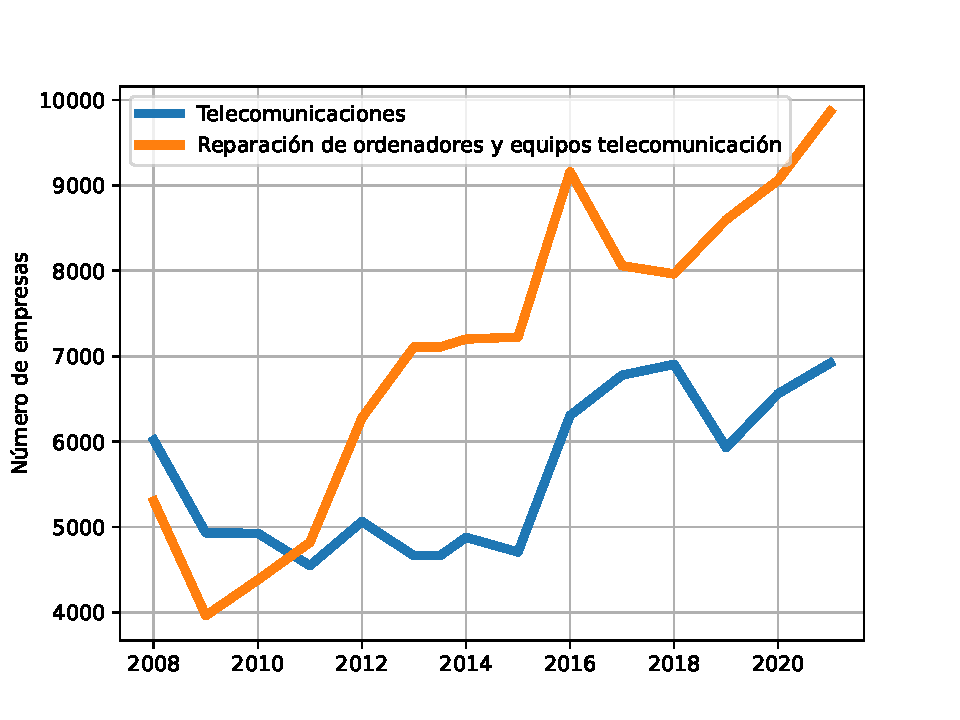
\includegraphics[width=.4\textwidth]{figures/crecimiento-tic-ine}
    \caption{Crecimiento empresarial de las TIC relacionadas con
    telecomunicaciones en España según el INE.}
    \label{fig:empresas-telco-ine}
\end{figure}

\end{frame}




\begin{frame}{\subsecname}
    Sobre la tecnología en el ámbito médico:
    \begin{itemize}
        \item 50\% de nuevos trabajos tras pandemia (WEF)
        % \item incremento 7.7\% y 2\% de inversión en sanidad
        %     en España y Madrid (FENIN)
        \item 32,000 empleos directos en 2023 (FENIN)
        \item 17º país con más trabajos en Eurozona (MedTech)
    \end{itemize}
\begin{figure}[t]
    \centering
    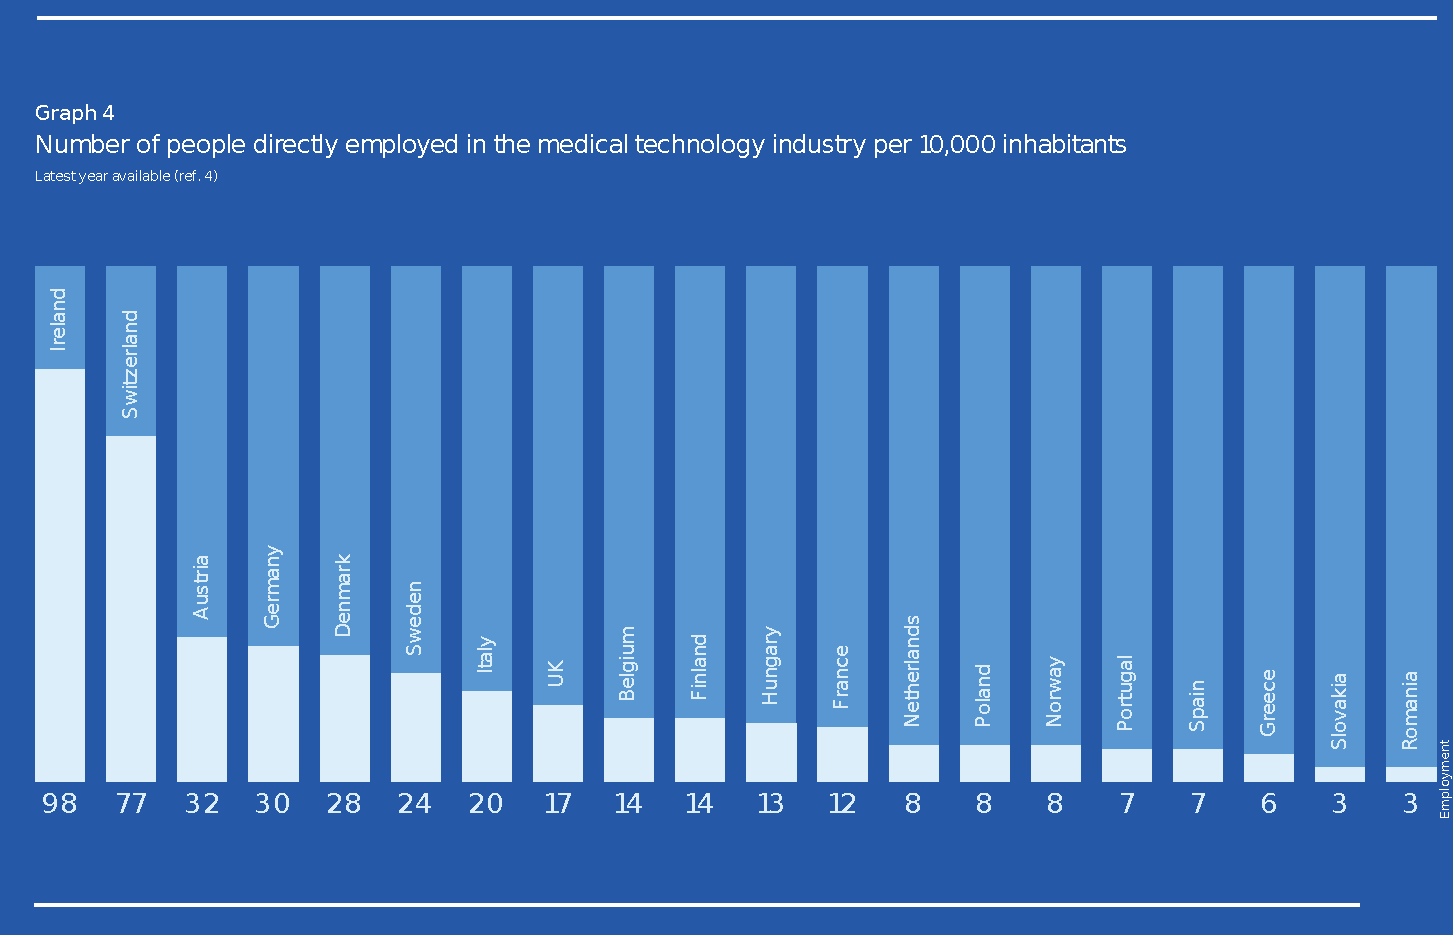
\includegraphics[width=.6\textwidth]{figures/medtech-europe--facts-figures-2024}
    \caption{Número de trabajadores tecnológicos en el
    ámbito médico en 2023 en la eurozona según
    MedTech.}
    \label{fig:medtech}
\end{figure}
\end{frame}



\subsection{Planificación y Técnicas Docentes}
\begin{frame}[allowframebreaks]{Contenido}
    \tableofcontents[currentsubsection]
\end{frame}

\begin{frame}{\subsecname}
    \begin{columns}[T] % align columns
\begin{column}{.48\textwidth}

Planificación:
\begin{itemize}
    \item aprendizaje basado en competencias -- EEES
    \item ECTS (26-27h) de trabajo en UPM
    \item resultados de aprendizaje en SET
    \item guías docentes/de aprendizaje
        \begin{itemize}
            \item objetivos
            \item competencias
            \item resultados de aprendizaje 
            \item cronograma 
        \end{itemize}
\end{itemize}

\end{column}%
\hfill%
\begin{column}{.48\textwidth}

\begin{figure}
    \small
    \vspace{-1em}
    \begin{tikzpicture}
        \node[rectangle,draw,fill=upmblue!20]
            (magistral) {Clase Magistral};
        \node[rectangle,draw,anchor=north]
            at (magistral.south) (invertida) {Clase Invertida};
        \node[rectangle,draw,anchor=north,fill=upmblue!20]
            at (invertida.south) (cooperativo)
            {Aprendizaje Cooperativo};
        \node[rectangle,draw,anchor=north]
            at (cooperativo.south) (problemas)
            {Aprendizaje Basado en Problemas};
        \node[rectangle,draw,anchor=north,fill=upmblue!20]
            at (problemas.south) (proyectos)
            {Aprendizaje Orientado a Proyectos};
        \node[rectangle,draw,anchor=north]
            at (proyectos.south) (gamificacion)
            {Gamificación};
        \node[rectangle,draw,anchor=north,fill=upmblue!20]
            at (gamificacion.south) (retos)
            {Aprendizaje Basado en Retos};
        \node[rectangle,draw,anchor=north]
            at (retos.south) (servicios)
            {Aprendizaje Basado en Servicios};
        \node[rectangle,draw,anchor=north,fill=upmblue!20]
            at (servicios.south) (investigacion)
            {Aprendizaje Basado en Investigación};
        \node[rectangle,draw,anchor=north]
            at (investigacion.south) (design)
            {Design Thinking};
    \end{tikzpicture}
    \caption{Técnicas docentes.}
\end{figure}

\end{column}%
\end{columns}
\end{frame}





%%%%%%%%
% RSER %
%%%%%%%%
\subsection{Redes y Servicios}
\begin{frame}[allowframebreaks]{Contenido}
    \tableofcontents[currentsubsection]
\end{frame}
\begin{frame}{\subsecname}
    \begin{table}
        \begin{tabular}{ p{2cm} | p{7cm}}
            \toprule
            \rowcolor{upmblue!20}Créditos & 4 ECTS\\
            Titulación & Grado en Ingeniería Biomédica\\
            \rowcolor{upmblue!20}Curso & 4º curso\\
            Semestre & 1\textsuperscript{er} semestre\\
            \rowcolor{upmblue!20}Módulo &  Aplicaciones en Salud Digital\\
            Centro & ETSIT\\
            \rowcolor{upmblue!20}Estudiantes & 15 (2024-2025)\\
            Carácter & Optativa/Obligatoria \newline Itinerario Ingeniería de Datos y Salud Digital\\
            \bottomrule
        \end{tabular}
    \end{table}
\end{frame}




\begin{frame}{\subsecname}

\begin{itemize}
    \item Conocimiento previo: \emph{Redes y Comunicaciones}
\end{itemize}

\begin{figure}[t]
    \centering
    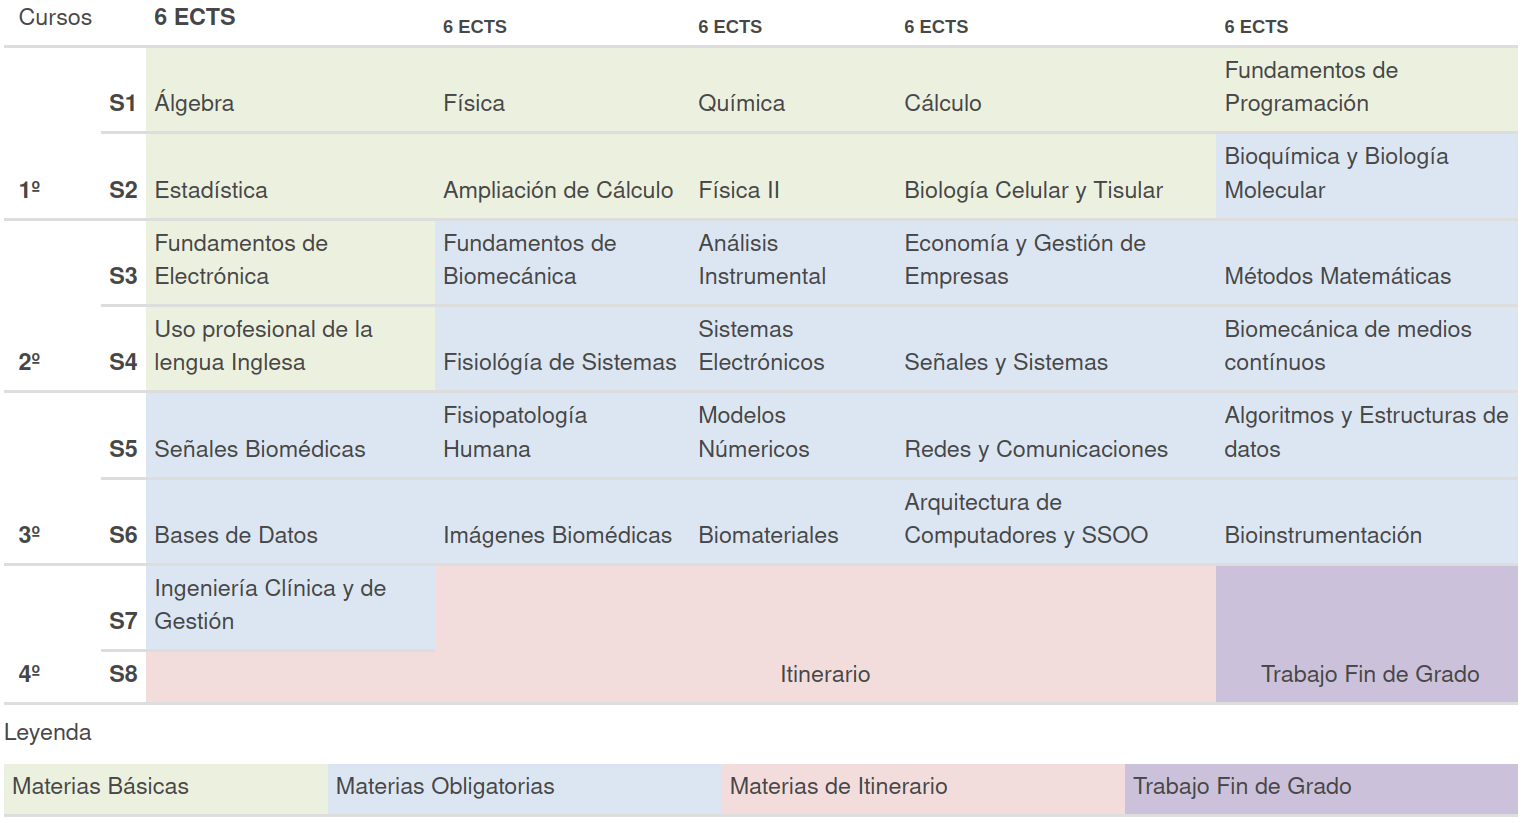
\includegraphics[width=.9\textwidth]{figures/gib-plan-estudios}
    \caption{Plan de estudios del Grado en Ingeniería Biomédica.}
    \label{fig:gib-plan-estudios}
\end{figure}

\end{frame}





\begin{frame}{\subsecname}

Módulos del plan de estudios:
\begin{itemize}
    \item \emph{Básico}: 60~ECTS
    \item \emph{Obligatorio}: 124~ECTS
    \item \emph{Optativo}: 32~ECTS itinerario + 12~ECTS
        optativas/prácticas
    \item \emph{TFG}: 12~ECTS
\end{itemize}
        

\begin{figure}[t]
    \centering
    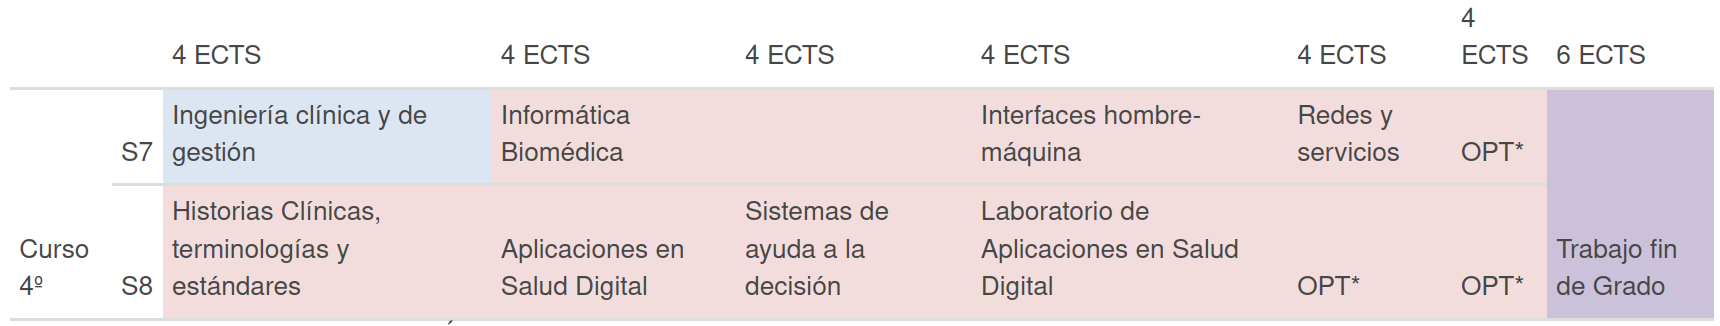
\includegraphics[width=.9\textwidth]{figures/gib-itinerario-datos}
    \caption{Itinerario en Ingeniería de Datos y Salud Digital.}
    \label{fig:gib-itinerario-datos}
\end{figure}

\end{frame}






\begin{frame}{\subsecname}
    Las competencias cubiertas son las siguientes
    \begin{itemize}
        \item \emph{CE25}: Conocer los principales sistemas de comunicaciones por cable e inalámbricos.
        \item \emph{CE26}: Conocer las redes de comunicaciones y su uso en los sistemas de gestión intra e interhospitalaria.
        \item \emph{CG03}: Ser capaz de manejar todas las tecnologías de la información y las comunicaciones
    \end{itemize}
\end{frame}



\begin{frame}{\subsecname}
    \begin{table}
        \centering
        \small
        \begin{tabular}{p{.8cm} | p{3.25cm} | p{4.7cm} | p{.8cm} }
            \toprule
            \textbf{Tema} & \textbf{Nombre} & \textbf{Contenido} & \textbf{Horas} \\ \midrule
            \rowcolor{upmblue!20} 1 &  Introducción a redes y servicios & Intro y protocolos de aplicación: DNS. & 2.5\\
            2 & Protocolos de mensajería entre dispositivos & MQTT publicación/suscripción, KEEPALIVE, cabeceras y QoS. & 15\\
            \rowcolor{upmblue!20}3 & Centros de datos & Definición, componentes, aplicaciones, requisitos. Eficiencia energética. Ejemplos de centros de datos.  Computación en la nube. Openstack. & 2.5\\
            4 & Nivel de red & Intro. Direcciones/prefijos IP. Reenvío. ICMP. NAT. & 7.5\\
            \rowcolor{upmblue!20}5 &  Redes de sensores  & Intro IoT, corto/medio/largo alcance (Bluetooth, WiFi Hallow, LoRaWAN). Redes (no)-IP: Gateways, 6LowPAN y Thread. & 5\\ \bottomrule
        \end{tabular}
    \end{table}
\end{frame}





\begin{frame}{\subsecname}
    Los resultados de aprendizaje son los siguientes:
    \begin{itemize}
        \item \emph{RA76:} Conocimientos teóricos y habilidades prácticas en las tecnologías necesarias para el desarrollo e
        integración de servicios de telemedicina.
        \item \emph{RA79:} Sabe aplicar las tecnologías de la información y las comunicaciones en todas las etapas del ciclo de vida.
        \item \emph{RA78:} Conocimiento del entorno en el que se han de instalar y operar los servicios de telemedicina.

        \item \emph{RA81:} Conoce un conjunto de métodos, tecnologías y recursos para el diseño, desarrollo y evaluación de
aplicaciones de telemedicina.
    \end{itemize}
\end{frame}




\begin{frame}{\subsecname}
    Técnicas docentes:
    \begin{itemize}
        \item \emph{Clase Magistral}: explicar
            conceptos básicos de la asignatura:
            MQTT, IP, centros de datos y redes de sensores.
        \item \emph{Aprendizaje Basado en Retos}:
            \begin{itemize}
                \item Mini-retos: sesiones de LAB para
                    asesorar y proponer escenarios de
                    mini-retos
                \item Reto capital: servicio de telemedicina
utilizando MQTT en redes IP para detectar anomalías
            \end{itemize}
    \end{itemize}
\end{frame}



\begin{frame}{\subsecname}
    \small
    \begin{itemize}

    \item Sesión \emph{LAB1}
            \begin{itemize}
                \item \emph{mini-reto}: uso mosquitto y capturas MQTT en wireshark.
            \end{itemize}

        \item Sesión \emph{LAB2} 
            \begin{itemize}
                \item\emph{mini-reto}: desarrollo de cliente MQTT servicio telemedicina
            \end{itemize}

\item Sesión \emph{LAB3}:
\begin{itemize}
    \item \emph{mini-reto}: despliegue broker MQTT
        + visualizar ctes. vitales
\end{itemize}


\item Sesión \emph{LAB4}
    \begin{itemize}
        \item \emph{mini-reto}: configurar red de transporte
            IP en VNX
    \end{itemize}


\item Sesión \emph{LAB5}
\begin{itemize}
    \item \emph{mini-reto}: APP detección de
        anomalías con suscriptor MQTT 
\end{itemize}


\item Sesión \emph{LAB6} 
\begin{itemize}
    \item \emph{reto capital}:
servicio de telemedicina
utilizando MQTT en redes IP para detectar anomalías
(integración)
\end{itemize}

\end{itemize}

\end{frame}




\begin{frame}{\subsecname}

\begin{table}
    \small
    \centering
\begin{tabular}{ p{3cm} | p{1.25cm} | p{3cm} | p{2cm} }
    \toprule
\textbf{Prueba} & \makecell{\bf Peso en \\ \bf la nota} & \makecell{\bf Competencias\\\bf evaluadas} & \makecell{\bf Resultados de \\\bf aprendizaje \\\bf evaluados} \\ \midrule
 \rowcolor{upmblue!20} Examen Parcial 1 & 40\% & CG3, CE25, CE26 & RA76, RA81 \\ 
Entrega LAB1 & 5\% & CG3, CE25, CE26 & RA78, RA79 \\ 
 \rowcolor{upmblue!20} Entrega LAB2 & 5\% & CG3, CE25, CE26 & RA78, RA79 \\ 
Entrega LAB3 & 5\% & CG3, CE25, CE26 & RA78, RA79 \\ 
 \rowcolor{upmblue!20} Entrega LAB4 & 5\% & CG3, CE25, CE26 & RA78, RA79 \\ 
Entrega LAB5 & 5\% & CG3, CE25, CE26 & RA78, RA79 \\ 
 \rowcolor{upmblue!20} Examen Parcial 2 & 10\% & CG3, CE25, CE26 & RA76, RA81 \\ 
Prueba de Integración & 25\% & CG3, CE26 & RA78, RA79 \\ \bottomrule
\end{tabular}
\caption{Evaluación de competencias en Redes y Servicios.}
\label{table:evaluacion-competencias-rser}
\end{table}
\end{frame}





\begin{frame}{\subsecname}
    \emph{RAID-BIO}: Red Avanzada para la Integración de Datos BIOmétricos en entornos hospitalario.
    \tikz[remember picture, overlay] {\node[anchor=north east] at ($(current page.north east)-(1,2)$) {
\includegraphics[width=1.5cm]{figures/logo-innovacion.png}};}
    \begin{itemize}
        \item Proyecto de innovación educativa 2025
        \item Aprendizaje basado en retos
        \item ODS3: Salud y Bienestar
            \begin{quote}
                \small
                suplir la insuficiencia de recursos disponibles en materia de recogida y
análisis de datos, así como de herramientas de simulación y alerta que permitan anticipar, controlar y gestionar situaciones
de riesgo para la salud pública
            \end{quote}
        \item compra dispositivos IoT para reporte biomédico
        \item reto global atajado por varios grados:
            \begin{itemize}
                \item GIB RSER: recolectar/proporcionar datos biomédicos
                \item GITST CDPS: tratamiento/visualización datos
                \item GISD RSTC: crear servicio distribuido
            \end{itemize}
    \end{itemize}

\end{frame}





\begin{frame}{\subsecname}
    \small

Bibliografía básica de la asignatura:


\begin{itemize}
    
    \item J. F. Kurose. Computer Networking, a top-down approach
    \item Labiod, H. Wi-Fi, Bluetooth, Zigbee And Wimax.
    \item Rob Barton. IoT Fundamentals: Networking Technologies, Protocols, and Use Cases for the Internet of Things
    \item  Gastón C. Hillar. MQTT Essentials - A Lightweight IoT Protocol
\end{itemize}
	

Bibliografía complementaria
\begin{itemize}
    \item Kevin Townsend. Getting Started with Bluetooth Low
Energy. 
    \item Chonggang Wang. ZigBee Network Protocols and Applications.
    \item  A. K. Bhoi.
5G IoT and Edge Computing for Smart Healthcare. 
\end{itemize}

Recursos de laboratorio:

\begin{itemize}
    \item Virtual Networks over linuX (VNX) web site. 
    \item Librería Paho MQTT. Cliente Mosquitto MQTT.
    \item Grafana: the open observability platform. Docker: Accelerated Container Application Development.
\end{itemize}
\end{frame}









%%%%%%%%
% RSTC %
%%%%%%%%
\subsection{Redes y Servicios de Telecomunicación}
\begin{frame}[allowframebreaks]{Contenido}
    \tableofcontents[currentsubsection]
\end{frame}
\begin{frame}{\subsecname}
    \begin{table}
        \begin{tabular}{ p{2cm} | p{7cm}}
            \toprule
            \rowcolor{upmblue!20}Créditos & 6 ECTS\\
            Titulación & Grado en Ingeniería de Tecnologías y Sistemas de Telecomunicación\\
            \rowcolor{upmblue!20}Curso & 2º curso\\
            Semestre & 2º semestre\\
            \rowcolor{upmblue!20}Competencias &  Formación Común\\
            Centro & ETSIT\\
            \rowcolor{upmblue!20}Estudiantes & 398 (2024-2025)\\
            Carácter & Obligatoria \\
            \bottomrule
        \end{tabular}
    \end{table}
\end{frame}




\begin{frame}{\subsecname}

\begin{itemize}
    \item Conocimiento previo:
        {\emph{Señales Aleatorias,
        Fundamentos de los Sistemas Telemáticos,
        Programación}}
    \item Asignaturas relacionadas:
        \tiny\emph{Redes de Ordenadores, Redes Corporativas,
        Redes de Comunicaciones Móviles,
        Centros de Datos y Provisión de Servicios,
        Redes y Servicios Radio, Dimensionado y Operación
        de Redes}
\end{itemize}

\begin{figure}[t]
    \centering
    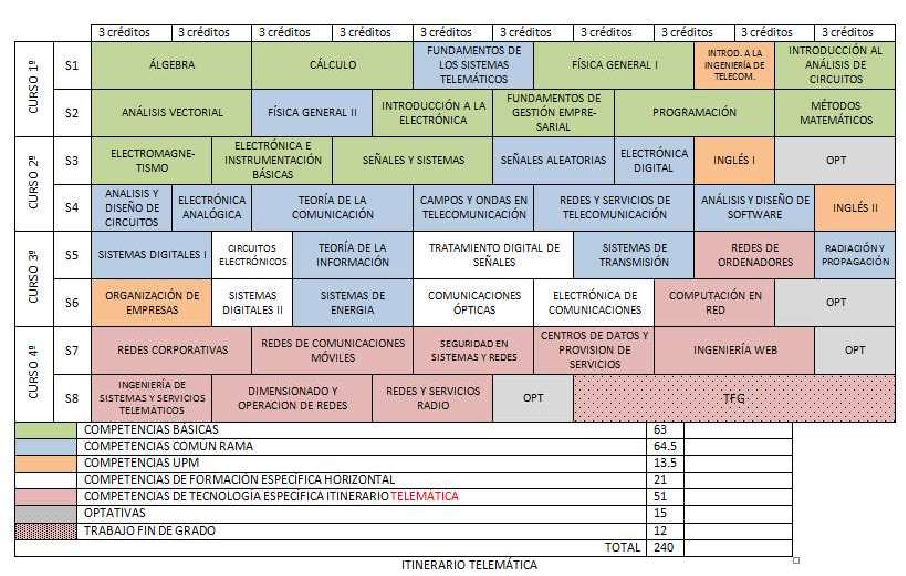
\includegraphics[width=.6\textwidth]{figures/rstc-plan-estudios}
    \caption{Plan de estudios del Grado en Tecnologías
    y Sistemas de Telecomunicación.}
    \label{fig:gib-plan-estudios}
\end{figure}

\end{frame}





\begin{frame}{\subsecname}

Módulos del plan de estudios:
\begin{itemize}
    \item \emph{Básica}:
        63~ECTS 
    \item \emph{Formación Común}: 64.5~ECTS
    \item \emph{Tecnología Específica}:
        48/51~ECTS
    \item \emph{Trabajo Fin de Grado}: 12~ECTS.
    \item \emph{Formación Específica Horizontal}:
        24/21~ECTS 
    \item \emph{Formación Transversal y Complementaria}:
        13.5~ECTS 
    \item \emph{Optativo}: 15~ECTS
\end{itemize}

        

\begin{figure}[t]
    \centering
    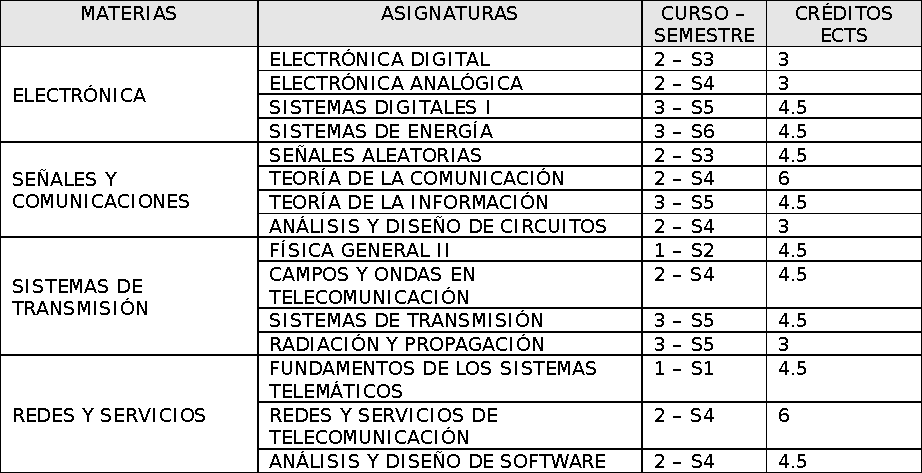
\includegraphics[width=.6\textwidth]{figures/gitst-modulo-comun}
\caption{Módulo Común}% del Grado en Sistemas y Tecnologías de Telecomunicación}
    \label{fig:gitst-modulo-comun}
\end{figure}

\end{frame}




\begin{frame}[allowframebreaks]{\subsecname}
    Las competencias adquiridas son
    \begin{itemize}
        \item \emph{CECT12}: Conocimiento y utilización de los conceptos de arquitectura de red, protocolos e interfaces de
comunicaciones
\item \emph{CECT13}: Capacidad de diferenciar los conceptos de redes de acceso y transporte, redes de conmutación de
circuitos y de paquetes, redes fijas y móviles, así como los sistemas y aplicaciones de red distribuidos, servicios de
voz, datos, audio, vídeo y servicios interactivos y multimedia.
\item \emph{CECT14}: Conocimiento de los métodos de interconexión de redes y encaminamiento, así como los fundamentos
de la planificación, dimensionado de redes en función de parámetros de tráfico
\item \emph{CECT15}: Conocimiento de la normativa y la regulación de las telecomunicaciones en los ámbitos nacional,
europeo e internacional
\item \emph{CECT2}: Capacidad de utilizar aplicaciones de comunicación e informáticas (ofimáticas, bases de datos, cálculo
avanzado, gestión de proyectos, visualización, etc.) para apoyar el desarrollo y explotación de redes, servicios y
aplicaciones de telecomunicación y electrónica.
\item \emph{CECT3}: Capacidad para utilizar herramientas informáticas de búsqueda de recursos bibliográficos o de
información relacionada con las telecomunicaciones y la electrónica
\item \emph{CECT6}: Capacidad de concebir, desplegar, organizar y gestionar redes, sistemas, servicios e infraestructuras de
telecomunicación en contextos residenciales (hogar, ciudad y comunidades digitales), empresariales o
institucionales responsabilizándose de su puesta en marcha y mejora continua, así como conocer su impacto
económico y social
\item \emph{CG1}: Que los estudiantes hayan demostrado poseer y comprender conocimientos en un área de estudio que
parte de la base de la educación secundaria general, y se suele encontrar a un nivel que, si bien se apoya en
libros de texto avanzados, incluye también algunos aspectos que implican conocimientos procedentes de la
vanguardia de su campo de estudio
\item \emph{CG12}: Organización y planificación
\item \emph{CG6}: Uso de la lengua inglesa
\item \emph{CG9}: Uso de Tecnologías de la Información y de las Comunicaciones
    \end{itemize}
\end{frame}







\begin{frame}{\subsecname}
    \begin{table}
        \centering
        \small
        \begin{tabular}{p{.7cm} | p{3.5cm} | p{4.75cm} | p{.8cm} }
            \toprule
            \textbf{Tema} & \textbf{Nombre} & \textbf{Contenido} & \textbf{Horas} \\ \midrule
            \rowcolor{upmblue!20} 1 &  Fundamentos de redes de comunicaciones & Encapsulado, PDU, prestaciones, cronogramas,
            recuperación de errores, red acceso xPON & 4\\
            2 &  Redes de Área Local & Nivel físico, formato tramas y direccionamiento, Ethernet, WiFi & 14\\
            \rowcolor{upmblue!20}3 & Redes de conmutación de paquetes  & Conmutación, Redes de conmutación de paquetes, redes IP. & 14\\
            4 &  Fundamentos de teletráfico y teoría de colas
              & Distribución exponencial/Poisson, M/M/1. & 12\\
            \rowcolor{upmblue!20}5 &  Teletráfico en redes de conmutación de paquetes & M/G/1, redes de Jackson. & 6 \\ 
            6 &   Modelos de teletráfico con pérdidas
              & M/M/N, M/M/1/K, M/M/N/N. & 8 \\ \bottomrule
        \end{tabular}
    \end{table}
\end{frame}




\begin{frame}{\subsecname}

Los resultados de aprendizaje son los siguientes
\begin{itemize}

\item \emph{RA51}: Conocimiento y aplicación de la normativa y regulación de protocolos y redes de los organismos internacionales de normalización (UIT-T, IETF, ETSI, IEEE802,..).

\item \emph{RA49}: Conocer modelos de arquitectura de protocolos.

\item  \emph{RA50}: Comprensión de mecanismos de protocolos TCP/IP y de métodos de encaminamiento/interconexión de redes.

\item \emph{RA47}: Comprensión de las tecnologías de conmutación y compartición de recursos.

\item \emph{RA48}: Capacidad de análisis de las prestaciones (retardo, probabilidad de perdidas, probabilidad de bloqueo, etc.) de una red de telecomunicación.

\item \emph{RA46}: Conocimiento de los componentes estructurales y funcionales de una red de telecomunicación y sus servicios fijos y móviles.

\end{itemize}
\end{frame}









\begin{frame}{\subsecname}
    Técnicas docentes:
    \begin{itemize}
        \item \emph{Clase Magistral}: explicar
            conceptos básicos de la asignatura:
            encapsulado, recuperación de errores,
            red acceso xPON, LAN, WiFi, formato de
            tramas, redes IP, sistemas M/M/1, M/G/1, etc.
            \begin{itemize}
                \item realización de
            Wooclaps en clases magistrales sobre los
            conceptos impartidos (1 por tema).
            \end{itemize}
        \item \emph{Resolución de problemas en clase}:
            los problemas se entregan en Moodle y resuelven
            en clase para solventar dudas.
    \end{itemize}
\end{frame}







\begin{frame}{\subsecname}


\begin{itemize}

    \item \emph{Práctica 1: conmutación Ethernet y STP}.
        \begin{itemize}
                \item Analizar tablas reenvío conmutadores Eth y análisis de STP.
    \end{itemize}
 
    \item \emph{Práctica 2: VLAN en una red Ethernet conmutada}.
        \begin{itemize}
            \item Configurar conmutadores Eth y despliegue
                VLAN con etiquetado de puertos.
        \end{itemize}

    \item \emph{Práctica 3: análisis de redes IP}.
        \begin{itemize}
            \item Configurar direccionamiento y reenvío IP
                en Linux. Distinguir entre nivel de red y enlace.
                Uso ping, traceroute, ip.
        \end{itemize}

    \item \emph{Práctica 4: simulación de redes de colas}.
        \begin{itemize}
            \item Simular sistemas M/M/1, M/M/K y redes
                de Jackson para
                verificar prestaciones y tiempo de convergencia
                cadena de Markov.
        \end{itemize}
  

\end{itemize}
\end{frame}









\begin{frame}{\subsecname}

\begin{table}
    \small
    \centering
\begin{tabular}{ p{3cm} | p{1.25cm} | p{3cm} | p{2cm} }
    \toprule
\textbf{Prueba} & \makecell{\bf Peso en \\ \bf la nota} & \makecell{\bf Competencias\\\bf evaluadas} & \makecell{\bf Resultados de \\\bf aprendizaje \\\bf evaluados} \\ \midrule
 \rowcolor{upmblue!20} Examen Parcial 1 & 55\% & CG9, CECT2,
CECT3, CECT6,
CECT12, CECT13,
CECT14, CG1 y CG6
 & RA47, RA46, RA49,
RA50, RA51 \\ 
 Examen Parcial 2 & 45\% & CG6, CG9, CG12,
CECT2, CECT3,
CECT6, CECT12,
CECT13, CECT14,
CECT15 y CG1
 & RA48
 \\ \bottomrule
\end{tabular}
\caption{Evaluación competencias Redes y Servicios de Telecomunicación.}
\label{table:evaluacion-competencias-rser}
\end{table}
\end{frame}














%%%% \begin{frame}{\subsecname}
%%%%     \emph{RAID-BIO}: Red Avanzada para la Integración de Datos BIOmétricos en entornos hospitalario.
%%%%     \tikz[remember picture, overlay] {\node[anchor=north east] at ($(current page.north east)-(1,2)$) {
\includegraphics[width=1.5cm]{figures/logo-innovacion.png}};}
%%%%     \begin{itemize}
%%%%         \item Proyecto de innovación educativa 2025
%%%%         \item Aprendizaje basado en retos
%%%%         \item ODS3: Salud y Bienestar
%%%%             \begin{quote}
%%%%                 \small
%%%%                 suplir la insuficiencia de recursos disponibles en materia de recogida y
%%%% análisis de datos, así como de herramientas de simulación y alerta que permitan anticipar, controlar y gestionar situaciones
%%%% de riesgo para la salud pública
%%%%             \end{quote}
%%%%         \item compra dispositivos IoT para reporte biomédico
%%%%         \item reto global atajado por varios grados:
%%%%             \begin{itemize}
%%%%                 \item GIB RSER: recolectar/proporcionar datos biomédicos
%%%%                 \item GITST CDPS: tratamiento/visualización datos
%%%%                 \item GISD RSTC: crear servicio distribuido
%%%%             \end{itemize}
%%%%     \end{itemize}
%%%% 
%%%% \end{frame}





\begin{frame}{\subsecname}
    \small


Bibliografía:


\begin{itemize}


    \item J. F. Kurose. Computer Networking, a top-down approach.

    \item Larry L. Peterson, Bruce
S. Davie. {Computer Networks: A Systems
        Approach}.  
    
    \item Andrew S.
Tanembaun, Nick Feamster, David
Wetherall. {Computer Networks}.
    
    \item Pablo Serrano, José A. Hernández. {Una introducción amable a la Teoría de colas}.
    
\end{itemize}
	
	 


Recursos para sesiones de laboratorio:
\begin{itemize}
    \item Documentación de switches modelo DGS-2000-10 del fabricante D-LINK. 
    \item Manuales sobre los principales comandos de los sistemas Linux.
    \item Virtual Networks over linuX (VNX) web site. 
    \item Documentación del simulador Ciw.
\end{itemize}


\end{frame}







%%%%%%%%%%%%%%%%%%%%%%%%%
% PROYECTO INVESTIGADOR %
%%%%%%%%%%%%%%%%%%%%%%%%%


\section{Proyecto Investigador}
\subsection{Marco Legal y de Investigación}

\begin{frame}[allowframebreaks]{Contenido}
    \tableofcontents[currentsubsection]
\end{frame}


% -------- enumerate funding funds
%% \begin{frame}{\subsecname}
%%     Fuentes:
%%     \begin{itemize}
%%         \item Ley Orgánica 2/2023, de 22 de marzo, del Sistema Universitario.
%%         \item Espacio Europeo de Investigación (EEI)
%%             -- Horizonte Europa (ERC):
%%             \begin{itemize}
%%                 \item Ciencia excelente: starting,
%%                     consolidator, advanced, proof of concept,
%%                     synergy grants
%%                 \item Marie Skłodowska-Curie:
%%                     Doctoral Networks, Postdoctoral
%%                     Fellowships, Staff Exchanges,
%%                     COFUND
%%             \end{itemize}
%%         \item EEI -- Consejo Europeo de Investigación (ECI):
%%             \begin{itemize}
%%                 \item EIC Pathfinder, Transition,
%%                     Accelerator, STEP Scale Up
%%             \end{itemize}
%% 
%%         \item Plan Estatal de Investigación Científica y Técnica y de Innovación (PEICTI)
%% 
%%         \item Plan Regional de Investigación Científica e Innovación Tecnológica (PRICIT)
%% 
%%     \end{itemize}
%% \end{frame}




\begin{frame}{\subsecname}
    Fuentes revisadas: LOSU, {\color{upmblue}EEI},
    {\color{yellow!80!black}PEICTI}\footnote{Plan Estatal de Investig Científica y Técnica y de Innovación (PEICTI)}, {\color{red}PRICIT}\footnote{Plan Regional de Invesig Científica e Innovación Tecnológica (PRICIT)}.
    \begin{figure}
        \begin{tikzpicture}

            % European
            \node[draw,rectangle,fill=upmblue!10]
                (starting) {ERC Starting};
            \node[draw,rectangle,fill=upmblue!10,
                anchor=north] (consolidator)
                at (starting.south) {ERC Consolidator};
            \node[draw,rectangle,fill=upmblue!10,
                anchor=north] (advanced)
                at (consolidator.south) {ERC Advanced};
            \node[draw,rectangle,fill=upmblue!10,
                anchor=north] (poc)
                at (advanced.south) {ERC PoC};
            \node[draw,rectangle,fill=upmblue!10,
                anchor=north] (synergy)
                at (poc.south) {ERC Synergy};
            \node[draw,rectangle,fill=upmblue!40,
                anchor=north] (docnet)
                at (synergy.south) {MSC DocNet};
            \node[draw,rectangle,fill=upmblue!40,
                anchor=north] (postdoc)
                at (docnet.south) {MSC Postdoc};
            \node[draw,rectangle,fill=upmblue!40,
                anchor=north] (staff)
                at (postdoc.south) {MSC Staff Ex};
            \node[draw,rectangle,fill=upmblue!40,
                anchor=north] (cofund)
                at (staff.south) {MSC COFUND};

            % National
            \node[draw,rectangle,fill=yellow!20] (genco)
                at ($(starting.east)+(2.5,0)$) {Gen. Conocimiento};
            \node[draw,rectangle,fill=yellow!20,
                anchor=north] (priv)
                at (genco.south) {Colab Pub-Privada};
            \node[draw,rectangle,fill=yellow!20,
                anchor=north] (docind)
                at (priv.south) {Doc. Industriales};
            \node[draw,rectangle,fill=yellow!20,
                anchor=north] (intcollab)
                at (docind.south) {Colab. Internacional};
            \node[draw,rectangle,fill=yellow!20,
                anchor=north] (ryc)
                at (intcollab.south) {Ramón y Cajal};
            \node[draw,rectangle,fill=yellow!20,
                anchor=north] (jdc)
                at (ryc.south) {Juan de la Cierva};
            \node[draw,rectangle,fill=yellow!20,
                anchor=north] (tecnico)
                at (jdc.south) {Prog. Técnico I+D};
            \node[draw,rectangle,fill=yellow!20,
                anchor=north] (consol)
                at (tecnico.south) {Consolidación Inv.};
            \node[draw,rectangle,fill=yellow!20,
                anchor=north] (redes)
                at (consol.south) {Redes Investigación};



            % Regional
            \node[draw,rectangle,fill=red!20] (talento)
                at ($(genco.east)+(2.5,0)$) {Prog. Talento};
            \node[draw,rectangle,fill=red!20,
                anchor=north] (cienciacon)
                at (talento.south) {Prog. Ciencia y Cono.};
            \node[draw,rectangle,fill=red!20,
                anchor=north] (colabval)
                at (cienciacon.south) {Prog. Colab. y valora.};
            \node[draw,rectangle,fill=red!20,
                anchor=north] (empresa)
                at (colabval.south) {Prog. I+C empresa.};
            \node[draw,rectangle,fill=red!20,
                anchor=north] (difpar)
                at (empresa.south) {Prog. Difu. Participa};
            \node[draw,rectangle,fill=red!20,
                anchor=north] (resultados)
                at (difpar.south) {Prog. Orient. Resultados};

        \end{tikzpicture}
    \end{figure}

\end{frame}







\subsection{Propuesta de Investigación}
\begin{frame}[allowframebreaks]{Contenido}
    \tableofcontents[currentsubsection]
\end{frame}




\begin{frame}{\subsecname}
    \textbf{Gestor Autónomo de Redes xG Usando el Contínuo Ciber-Físico.\footnote{xG: redes LTE, NR, 6G, 802.11p/bd.}\footnote{Contínuo cíber-físico: datos del mundo real y de red.}}
\vfill
\begin{figure}[t]
    \centering
    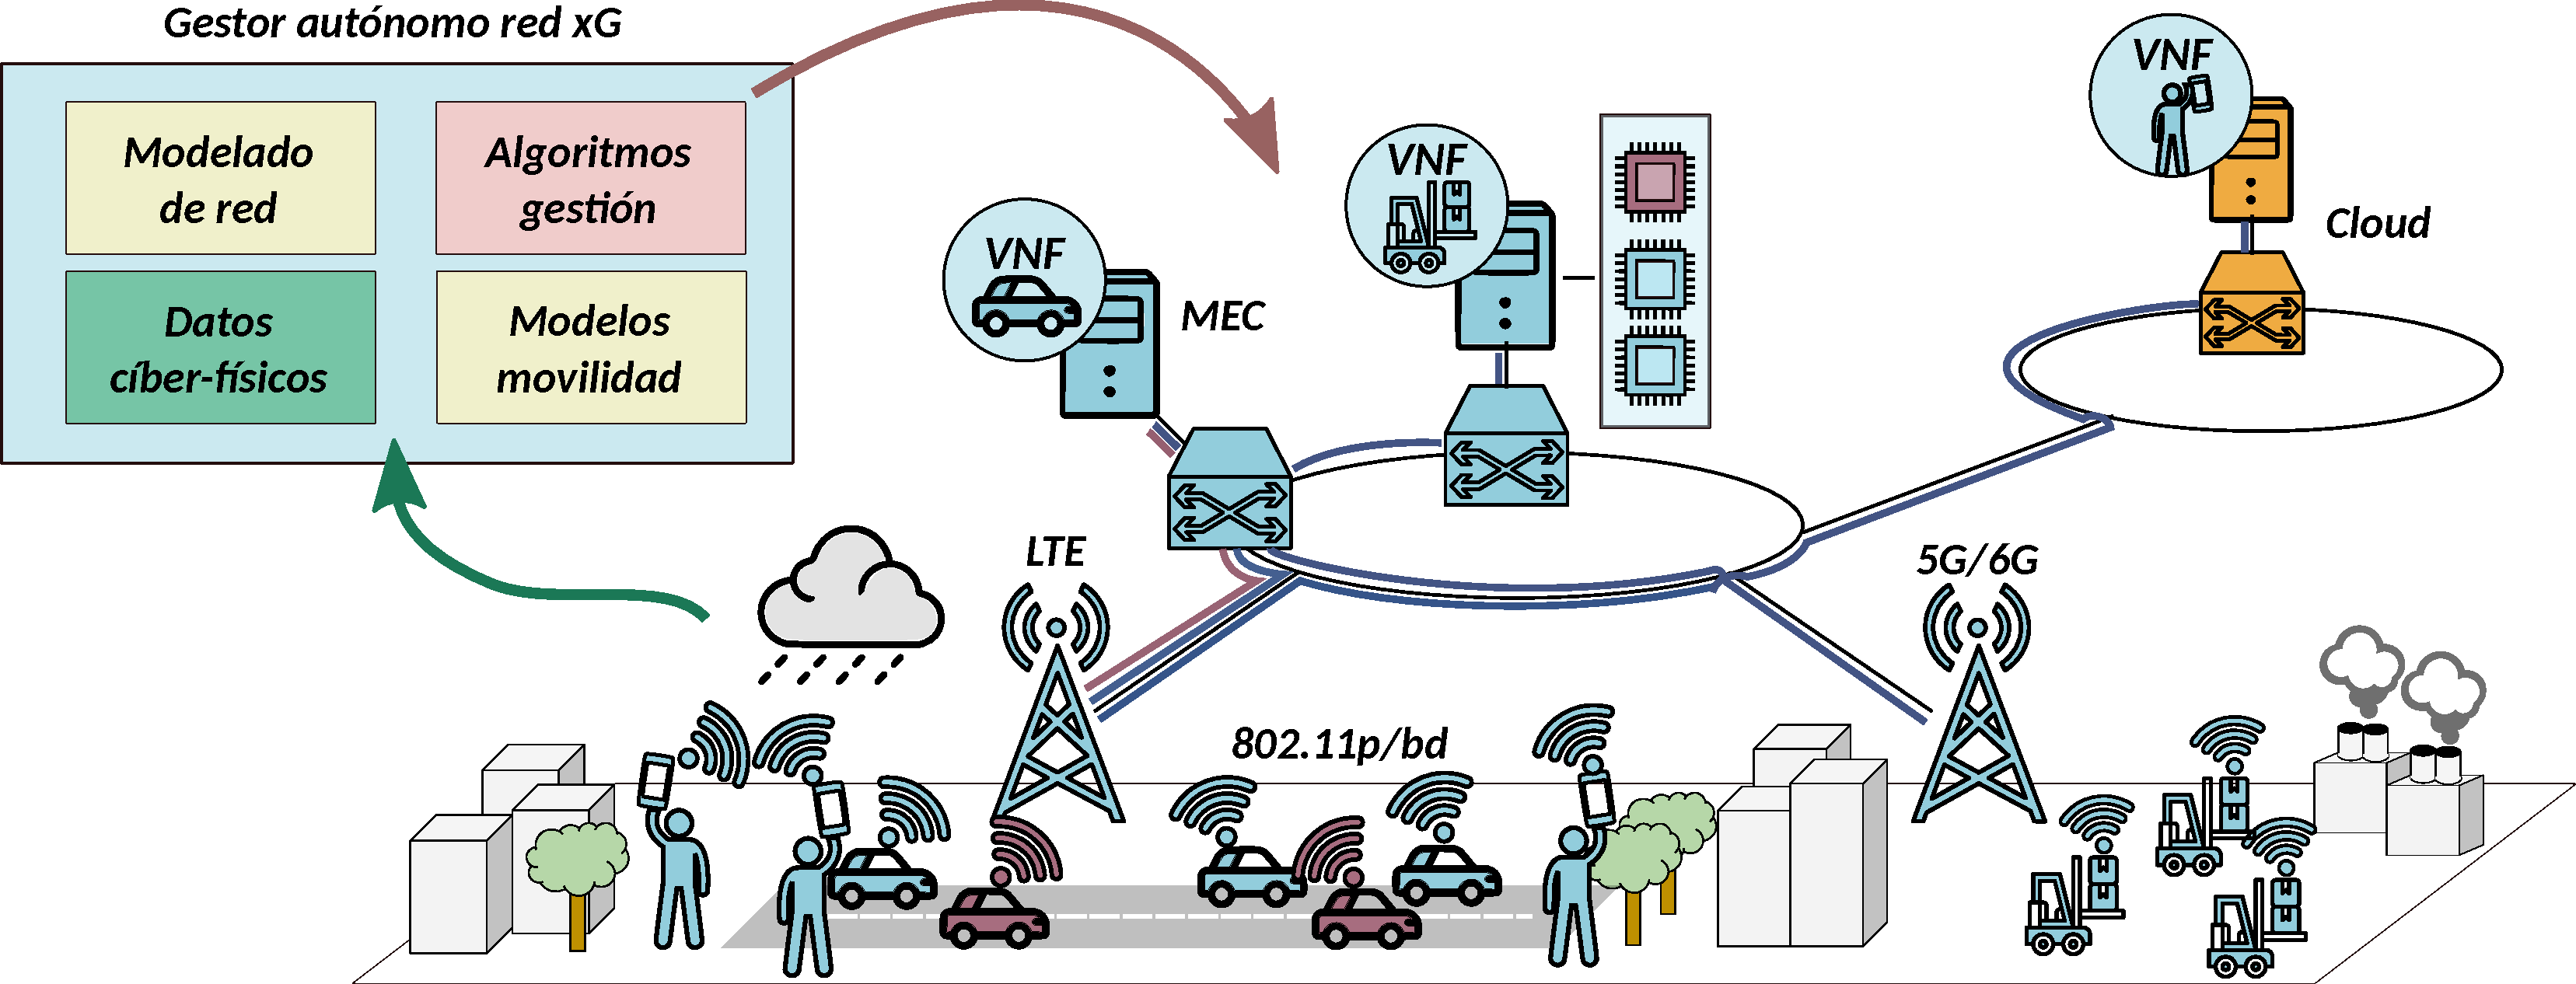
\includegraphics[width=\textwidth]{figures/big-picture-final-huge.pdf}
    \caption{El gestor autónomo xG recolectará
    información del contínuo cíber-físico para realizar
    labores de gestión de la RAN, red de transporte
    y recursos de cómputo.}
\end{figure}
\end{frame}



\subsection{Objetivos, Novedad y Etapas}
\begin{frame}[allowframebreaks]{Contenido}
    \tableofcontents[currentsubsection]
\end{frame}


\begin{frame}{\subsecname}
            Objetivos y resultados esperados:
            \begin{itemize}
                \item \emph{O1}: identificar interfaces de gestión y fuentes de intercambio de datos
                \item \emph{O2}: modelado de patrones de movilidad
                \item \emph{O3}: modelado de latencia en redes xG
                \item \emph{O4}: diseño de algoritmos para la gestión de redes xG
                \item \emph{O5}: validación en plataforma RAN y P4
            \end{itemize}
            \begin{figure}[t]
                \centering
                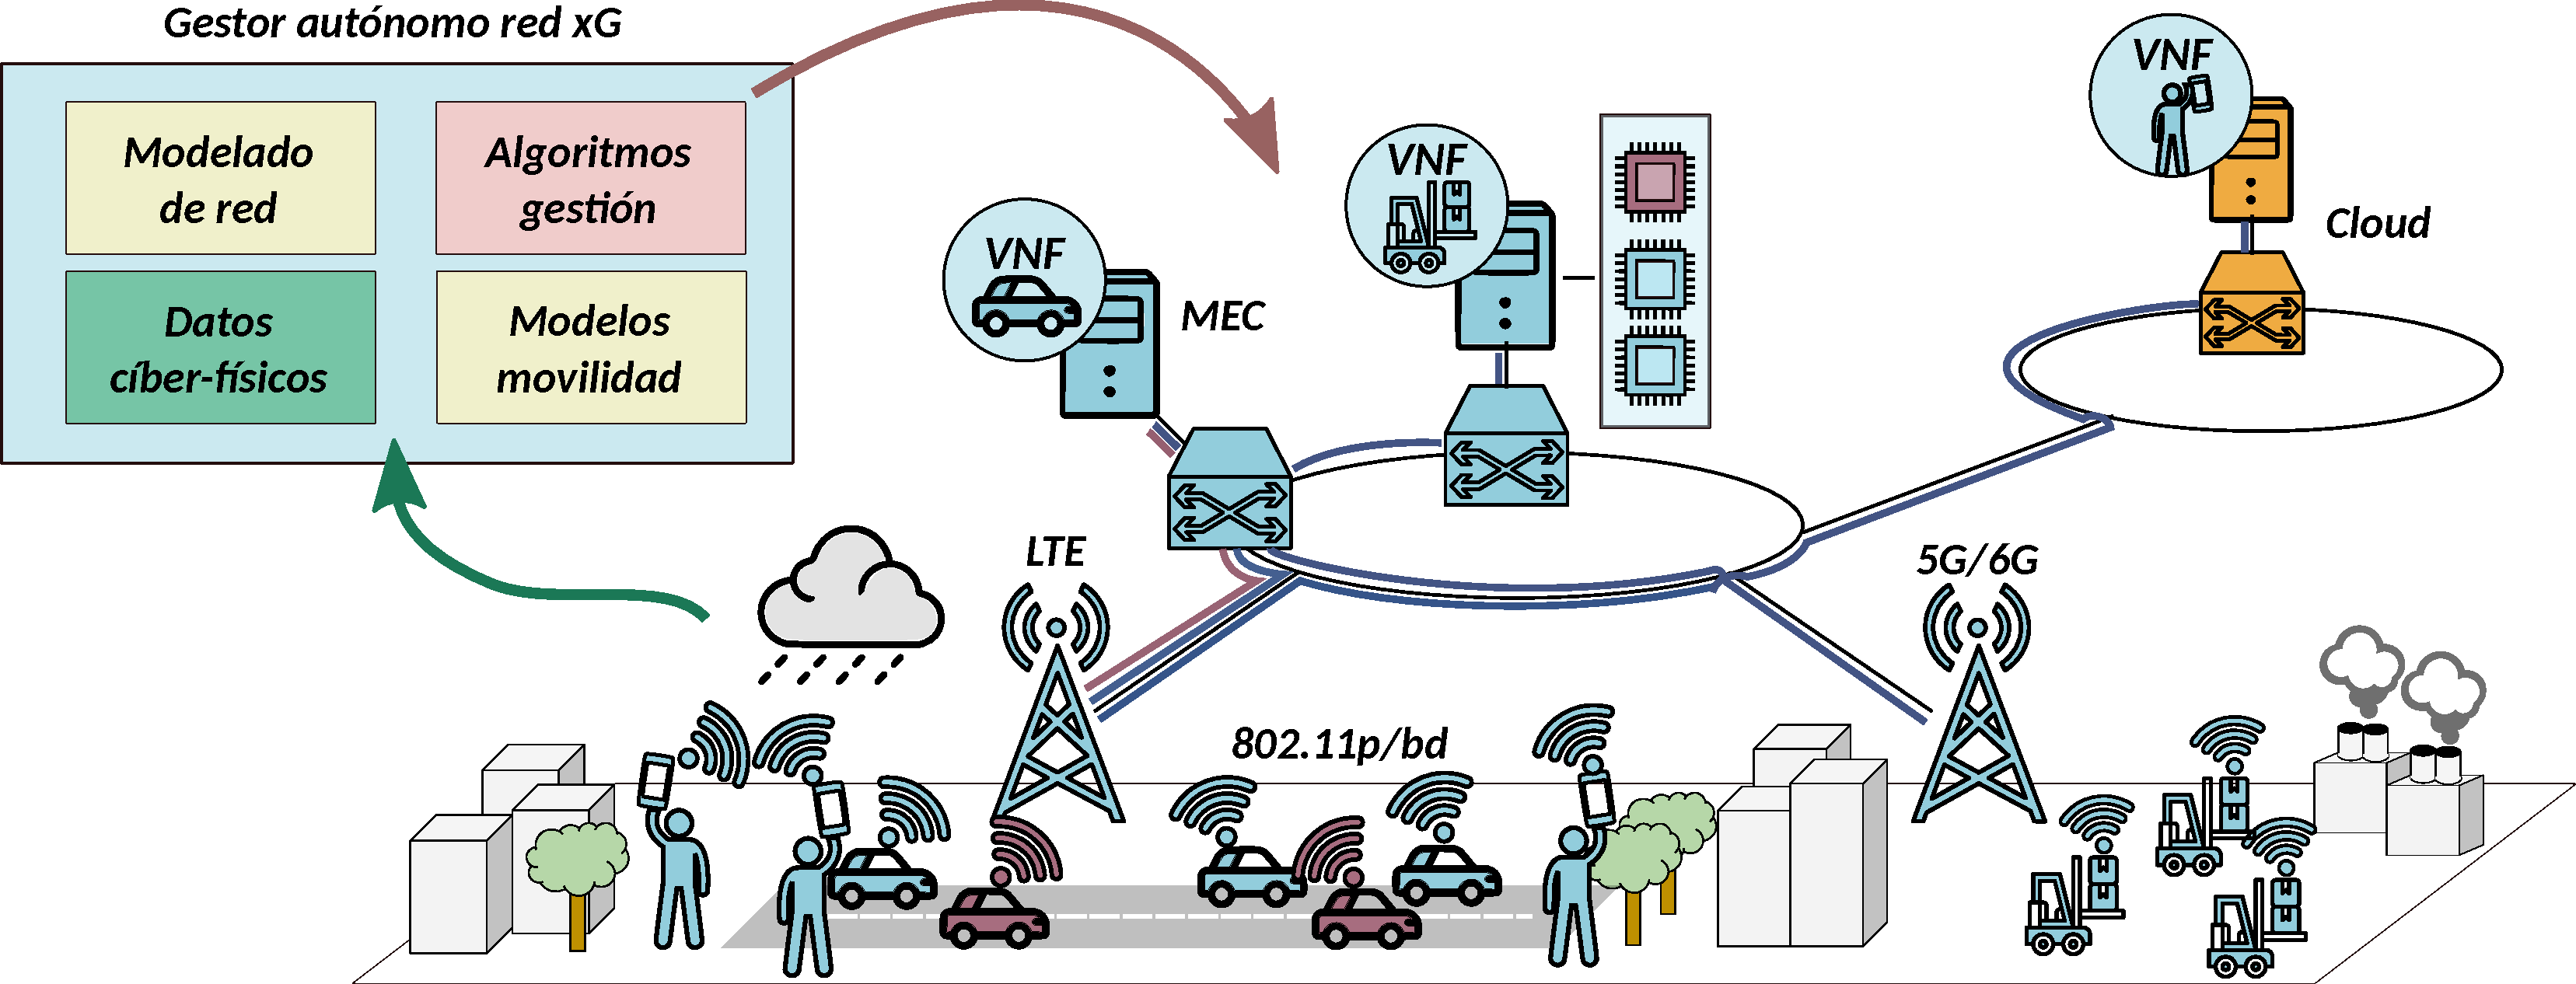
\includegraphics[width=.5\textwidth]{figures/big-picture-final-huge.pdf}
            \end{figure}
\end{frame}





\begin{frame}{\subsecname}
    Novedad del proyecto:
    \begin{enumerate}
        \item Crear una \emph{arquitectura} para
            gestionar xG usando datos del \emph{contínuo
            cíber-físico} (el tiempo, tráfico carretera,
            telemetría de red, etc.)
        \item Incorporar \emph{modelos de movilidad} para
            provisionamiento xG
        \item Uso de \emph{cálculo estocástico de redes}
            para modelado punto a punto (con movilidad)
        \item Uso de \emph{teoría espectral de grafos} para
            capacidad de V2X
        \item Uso de \emph{Optimización
            Clásica y Online (IA/ML)} para proveer
            de garantías de gestión en vivo
    \end{enumerate}
\end{frame}




\begin{frame}{\subsecname}
\begin{figure}[t]
    \centering
    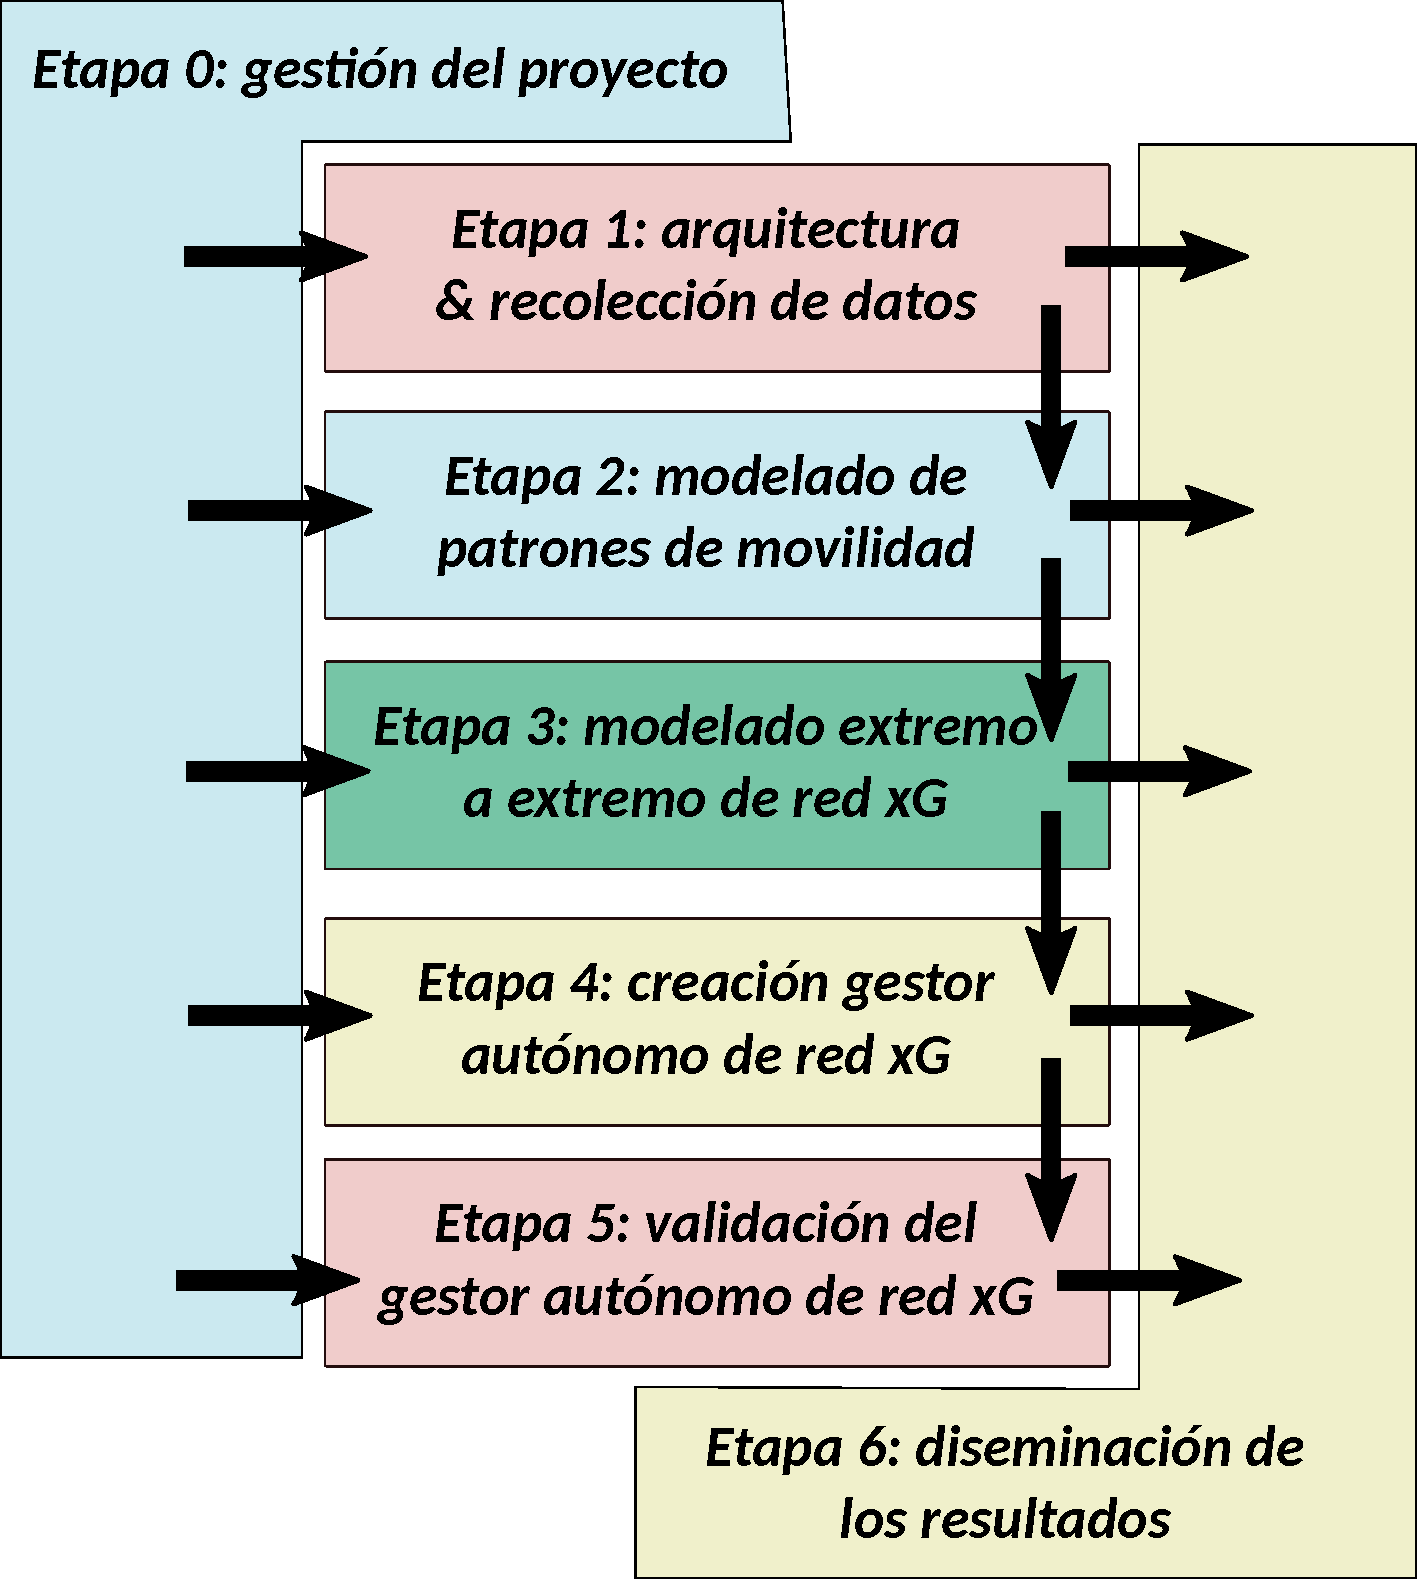
\includegraphics[width=.5\textwidth]{figures/etapas}
    \caption{Etapas de la propuesta de investigación.}
    \label{fig:etapas}
\end{figure}
\end{frame}



\begin{frame}{\subsecname}
    \begin{itemize}
        \item \emph{Etapa 0}: gestión del proyecto.
            \begin{itemize}
                \item gestión de hitos, fondos y personal.
                    % becas talento, concursos de financiación
            \end{itemize}
        \item \emph{Etapa 1}: arquitectura y recolección
            de datos.
            \begin{enumerate}
                \item identificar interfaces RAN
                    de recolección de datos (privacidad)
                \item identificar info. en VAMs/CAMs (privacidad)
                \item identificar interfaces almacenado
                    datos cíber-físicos DT
                \item identificar interfaces gestión red xG
            \end{enumerate}
    \end{itemize}

    \begin{figure}
        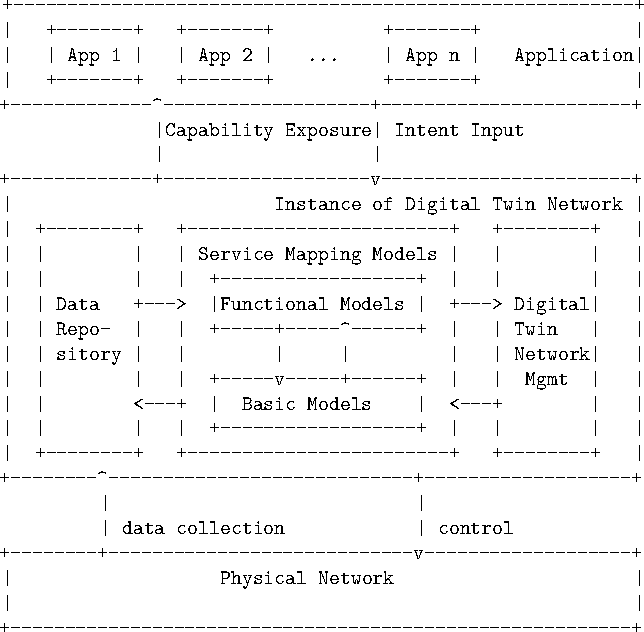
\includegraphics[width=.3\textwidth]{figures/digital-twin}
        \caption{Arquitectura IETF de un gemelo digital.}
    \end{figure}
\end{frame}





\begin{frame}{\subsecname}

    \begin{columns}[T] % align columns
        \begin{column}{.48\textwidth}



            \begin{itemize}
                \item \emph{Etapa 2}: modelado de patrones de
                    movilidad
                    \begin{enumerate}
                        \item estudio de modelos de movilidad:
                            PDEs, vector-based
                        \item codificación de modelos de
                            movilidad vehiculares y de peatones
                    \end{enumerate}
            \end{itemize}


            \begin{figure}[t]
                \centering
                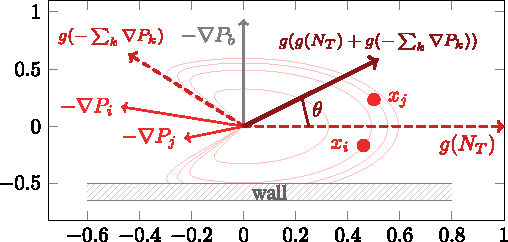
\includegraphics[width=.8\textwidth]{figures/isolines.pdf}
                \caption{Movilidad peatón.}
            \end{figure}


        \end{column}
        \begin{column}{.48\textwidth}
            \begin{itemize}
                \item \emph{Etapa 3}: modelado extremo a extremo
                    red xG
                \begin{enumerate}
                    \item modelado RAN: SNC
                    \item modelado transp: SNC 
                    \item modelado procesamiento
                    \item capacidad holística SGT
                \end{enumerate}
            \end{itemize}

            \vspace{2em}


            \begin{figure}[t]
                \centering
                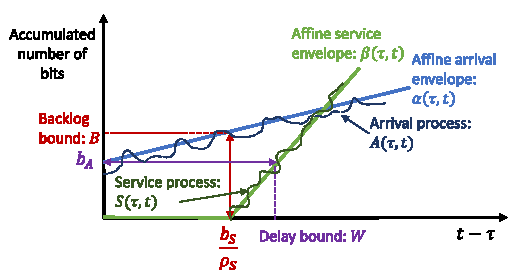
\includegraphics[width=.8\textwidth]{figures/snc.pdf}
                \vspace{-.5em}
                \caption{SNC.}
            \end{figure}
        \end{column}
    \end{columns}
\end{frame}




\begin{frame}{\subsecname}
    \begin{itemize}
        \item \emph{Etapa 4}: creación del gestor autónomo de redes xG
            \begin{enumerate}
                \item Gestión PUSCH/PDSCH de la RAN
                \item Conformado y enrutamiento
                    red transporte
                \item Escalado de recursos de cómputo para QoS
                \item Búsqueda de rutas de vehículos con QoS para V2X
            \end{enumerate}
    \end{itemize}



\begin{figure}
    \centering
    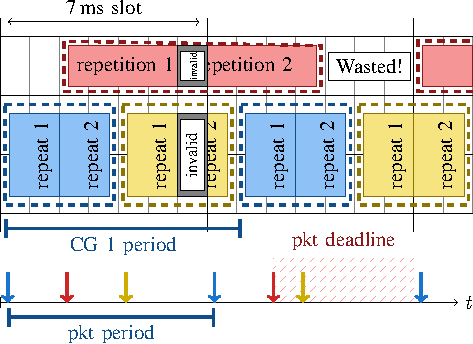
\includegraphics[width=.4\textwidth]{figures/configured-grant-repetitions.pdf}
    \caption{Reserva PUSCH con CG y repeticiones Tipo~B
    para URLLC.}
\end{figure}
\end{frame}






\begin{frame}{\subsecname}

    \begin{columns}[T] % align columns
        \begin{column}{.48\textwidth}



            \begin{itemize}
                \item \emph{Etapa 5}: validación del
                    gestor autónomo de la red xG
                    \begin{enumerate}
                        \item gestión de la RAN
                        \item gestión red de transporte
                        \item gestión de recursos de cómputo
                        \item gestión extremo a extremo
                    \end{enumerate}
            \end{itemize}




        \end{column}
        \begin{column}{.48\textwidth}
            \begin{itemize}
                \item \emph{Etapa 6}: diseminación de
                    resultados
                \begin{enumerate}
                    \item publicación científica
                    \item diseminación en medios
                    \item participación en ferias/eventos
                        de divulgación
                \end{enumerate}
            \end{itemize}
        \end{column}
    \end{columns}
    
    \begin{figure}[t]
        \centering
        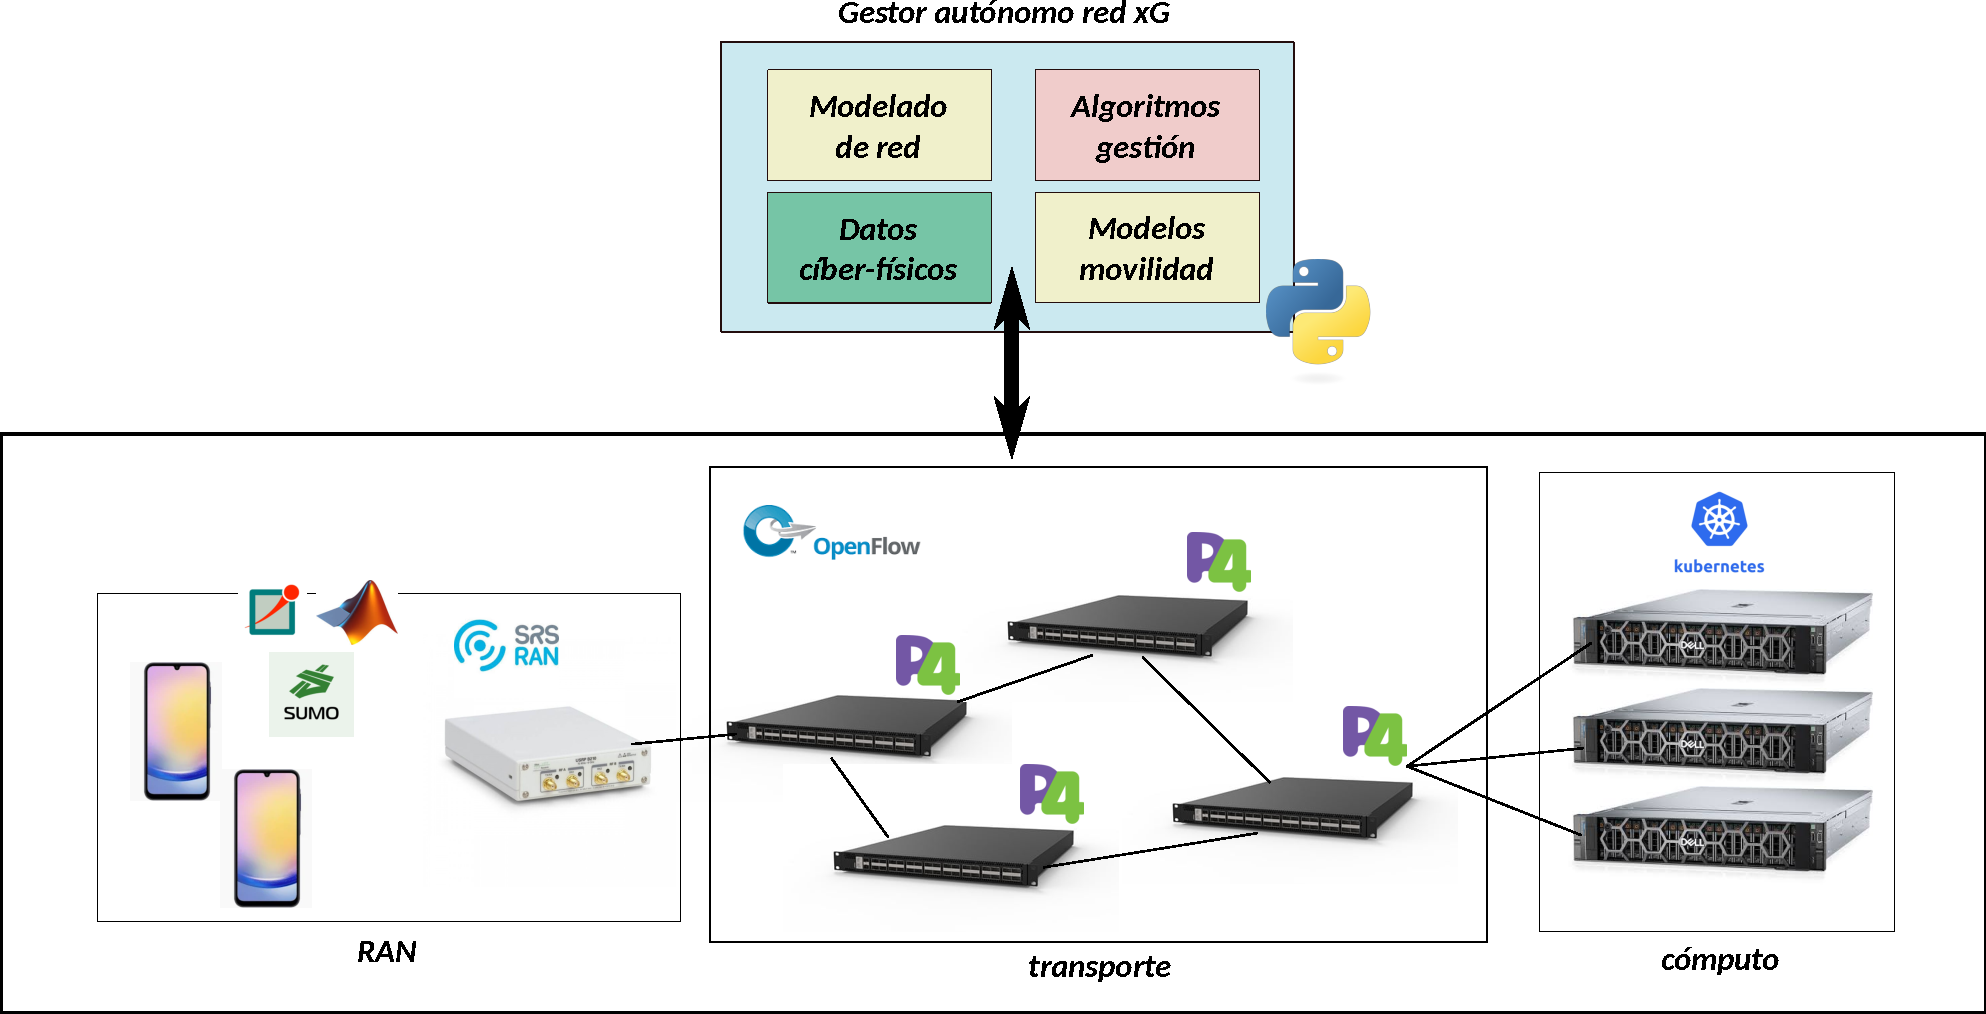
\includegraphics[width=.5\textwidth]{figures/validacion.pdf}
        \caption{Escenario de validación.}
    \end{figure}
\end{frame}






\begin{frame}{\subsecname}



%%%%% TABLA JORGE  ---  scaled effort
\definecolor{azulcielo}{rgb}{0.53, 0.81, 0.98}
\footnotesize
\begin{table}
\begin{adjustbox}{width=.7\textwidth,center}

\begin{tabular}{ p{12cm} | p{2cm}  } 

\toprule

{\bf Tarea} &  {\bf Personas/mes} \\ \hline

%% % Semana 1
%% \textbf{Presentación + Tema 1}. \newline Duración: 02:00 \newline
%% LM: Actividad del tipo Lección Magistral &
%% \textbf{Tema 1 (ejercicios)}\newline
%% Duración: 02:00\newline
%% PR: Actividad del tipo Clase de Problemas
%% & \\
%% \hline

\rowcolor{upmblue!20} \textbf{E0: gestión del proyecto} & \textbf{6} \\ \hline 
T0.1: Gestión de personal y fondos & 2 \\ \hline
T0.2: Gestión de hitos & 2 \\ \hline
T0.3:  Gestión de incumplimientos & 2 \\ \hline
% T0.4: Becas de talento & 1 \\ \hline
% T0.5: Concurso en convocatorias de financiación & 2 \\ \hline
 \rowcolor{upmblue!20} \textbf{E1: arquitectura y recolección de datos} & \textbf{12} \\ \hline 
T1.1: Identificar interfaces RAN de colección de datos & 4 \\ \hline
T1.2: Identificar información disponible en CAMs y VAMs & 4 \\ \hline
T1.3: Identificar interfaces y entidades de almacenamiento de datos y gestión. & 4 \\ \hline
 \rowcolor{upmblue!20}  \textbf{E2: modelado de patrones de movilidad} & \textbf{12} \\ \hline 
T2.1: Estudio del estado del arte en patrones de movilidad. & 7 \\ \hline
T2.2: Codificación de los modelos de movilidad. & 5 \\ \hline
 \rowcolor{upmblue!20}   \textbf{E3: modelado extremo a extremo de la red xG} & \textbf{25} \\ \hline 
T3.1: Modelado del medio inalámbrico. & 10 \\ \hline
T3.2: Modelado de la capa de transporte. & 5 \\ \hline
T3.3: Modelado de latencia de procesamiento. & 5 \\ \hline
T3.4: Capacidad holística de la red xG. & 5 \\ \hline
 \rowcolor{upmblue!20}   \textbf{E4: creación del gestor autónomo de redes xG} & \textbf{25} \\ \hline 
T4.1: Gestión del acceso RAN. & 10 \\ \hline
T4.2: Gestión de la red de transporte. & 5 \\ \hline
T4.3: Gestión de los recursos de procesado. & 5 \\ \hline
T4.4:  Gestión de rutas seguidas por vehículos que utilizan servicios V2X. & 5 \\ \hline
 \rowcolor{upmblue!20}   \textbf{E5: validación del gestor autónomo de la red xG} & \textbf{35} \\ \hline 
T5.1: Validación de gestión de la RAN. & 15 \\ \hline
T5.2: Validación de la gestión de la red de transporte. & 5 \\ \hline
T5.3:  Validación de la gestión de la infraestructura de cómputo. & 5 \\ \hline
T5.4:   Validación de la gestión extremo a extremo de una red xG. & 10 \\ \hline
 \rowcolor{upmblue!20}      \textbf{E6: diseminación de los resultados} & \textbf{5} \\ \hline 
T6.1: Publicación científica. & 2 \\ \hline
T6.2: Diseminación en medios. & 1 \\ \hline
T6.3: Participación en ferias/eventos de divulgación.  & 2 \\ \hline
 \rowcolor{upmblue!40}      \textbf{Total} & \textbf{120} \\ \bottomrule


\end{tabular}
\end{adjustbox}
\caption{Esfuerzo y dedicación a cada tarea en términos
de personas/mes.}
\label{tab:personas-mes}
\end{table}

\normalsize
%%%%%<- FIN TABLA JORGE


\end{frame}






\begin{frame}{\subsecname}
    \begin{figure}
    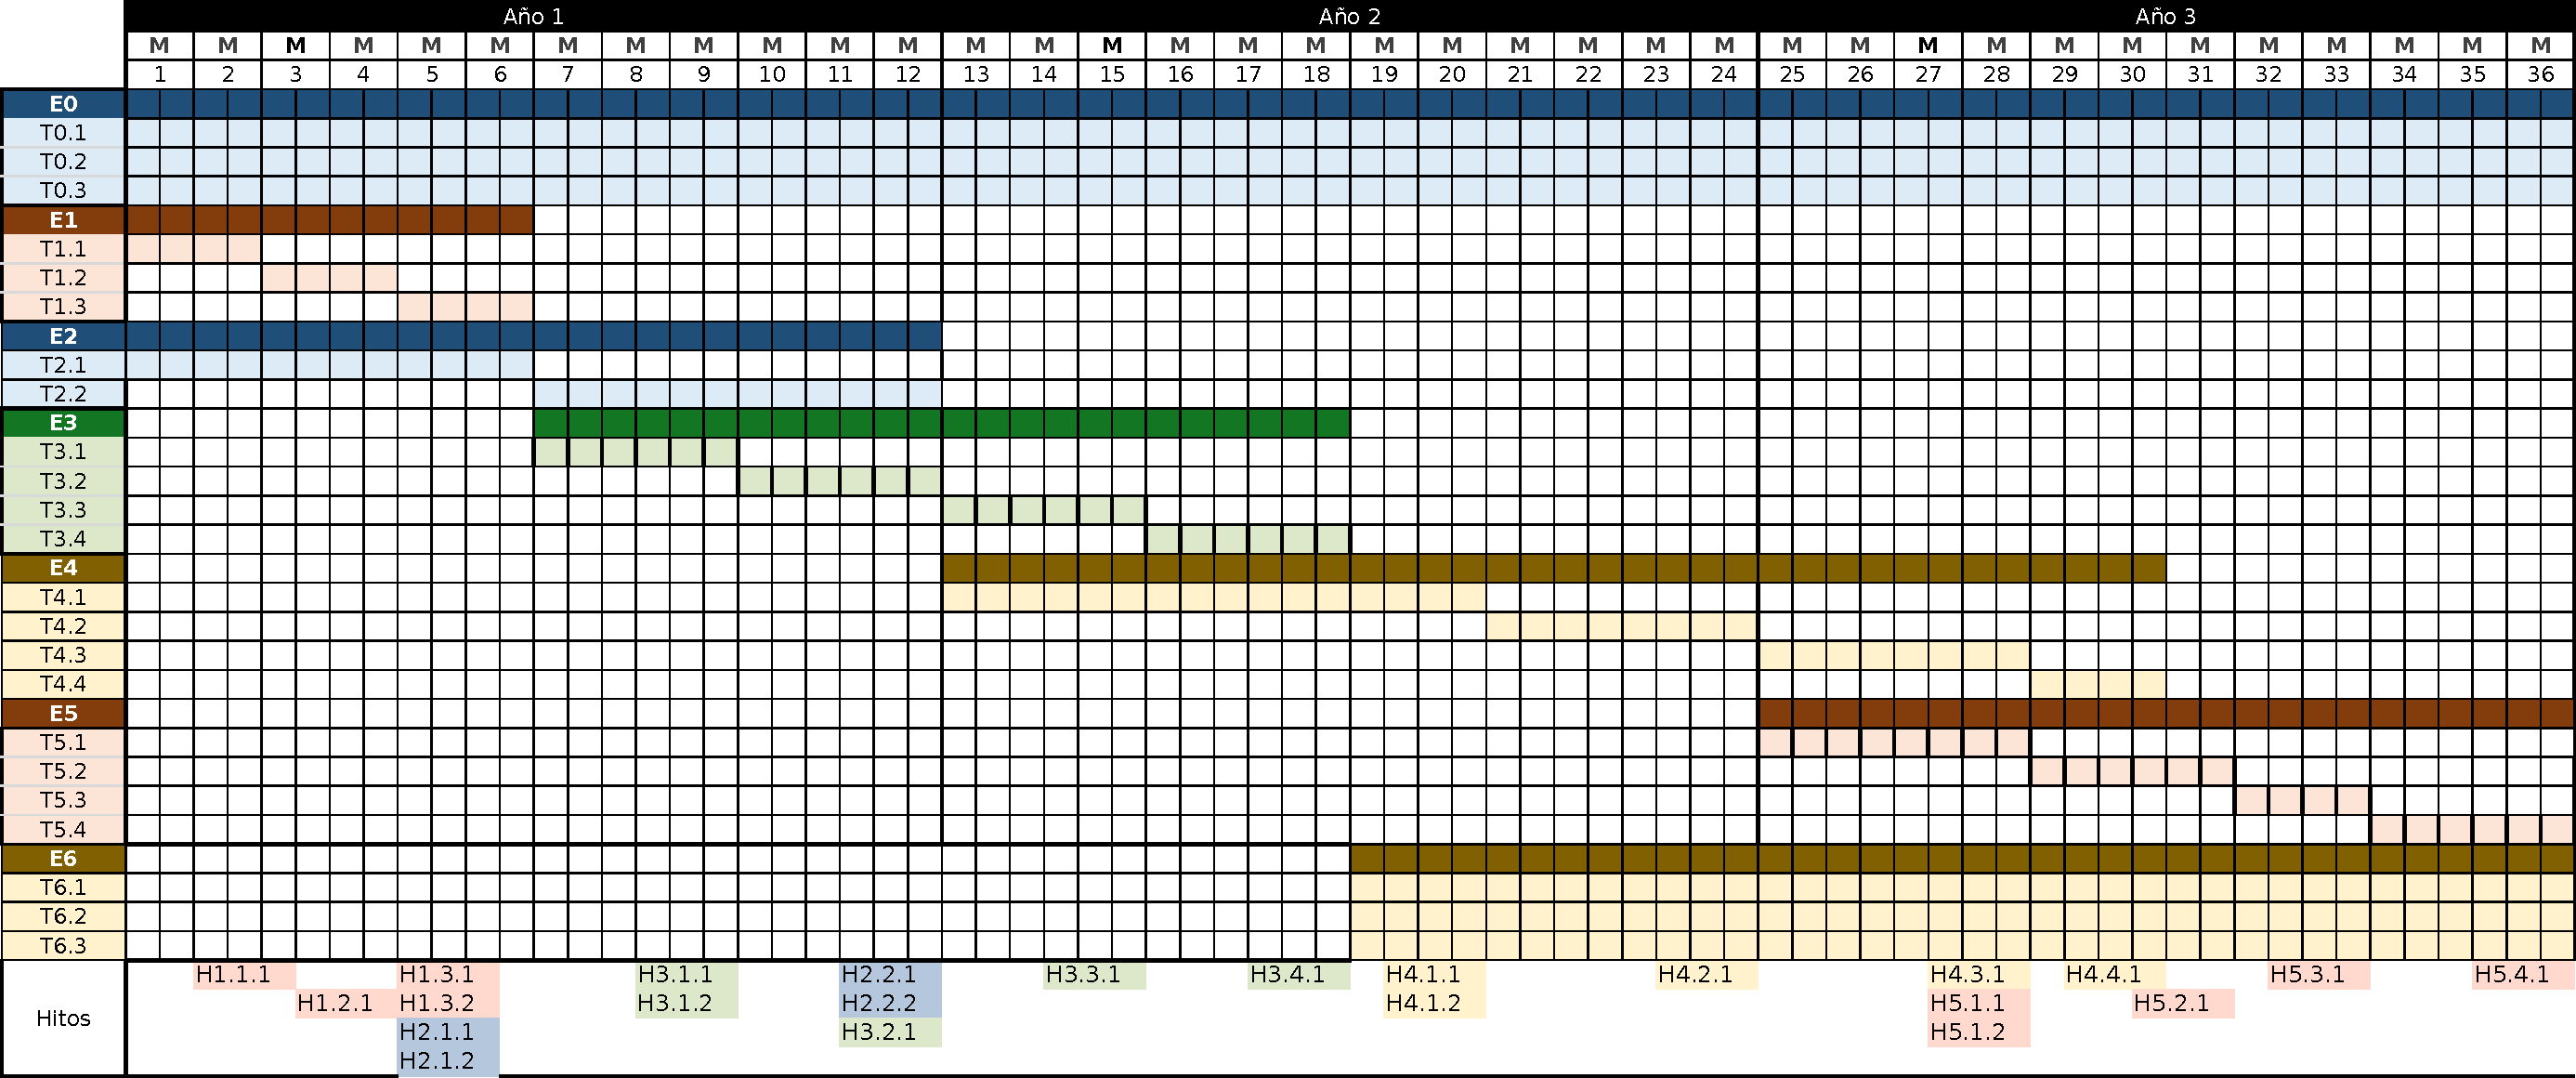
\includegraphics[width=\textwidth]{figures/ganttPPL.pdf}
    \caption{Diagrama de GANTT de la planificación del
    proyecto de investigación.}
    \end{figure}
\end{frame}





\begin{frame}{\subsecname}
    Intersección con proyectos @GIROS:
    \begin{itemize}
        \item Remote Driver (finalización 2025):
            \begin{itemize}
                \item NOKIA
                \item búsqueda de rutas de
                    vehículos con QoS para
                    conducción remota (V2N)
            \end{itemize}
        \item Across (finalización 2025):
            \begin{itemize}
                \item Telefónica
                \item rutas óptimas (energía) en red
                    de transporte
            \end{itemize}
        \item DISCO6G-CM (finalización 2028):
            \begin{itemize}
                \item UPM, UC3M, UAM, IMDEA Networks, 
                \item mejorar posicionamiento VAMs/CAMs
            \end{itemize}
    \end{itemize}
\end{frame}




\begin{frame}
\titlepage
\end{frame}

\end{document}
